% options are:
% PhD, MSc (choose one)
% beforeExam (to make the personal thanks invisible)
\documentclass[MSc,beforeExam]{iitcsthesis}

\usepackage{times}
\usepackage{latexsym}
\usepackage{graphicx} % more modern
\usepackage{graphics}
\usepackage{subfigure}
\usepackage{natbib}

\usepackage{algorithm}
\usepackage{hyperref}

\usepackage{amsfonts}
\usepackage{amsmath}
\usepackage{amstext}
\usepackage{latexsym}
\usepackage{amssymb}
\setcounter{tocdepth}{3}
\usepackage{epstopdf}
\usepackage{url}
\usepackage{color}
\usepackage{wrapfig}
\usepackage{fancyvrb}
\usepackage{rotating}
\usepackage{enumerate}
\usepackage{tabulary}

\usepackage[table]{xcolor}
%\usepackage{algpseudocode}
%\usepackage{algorithmic}


% For some reason, the hebrew package clashes with the amsthm package. If you need a proof environment, you can uncomment the following:
%\usepackage{amssymb} %Needed for \blacksquare. Take care not to add this package twice...
%\newenvironment{proof}[1][Proof]{\par \textbf{#1.} }{\hspace{10pt}\hfill$\blacksquare$\par}
\begin{document}

\authorEnglish{Haim Cohen}

\titleEnglish{Multi-task Learning with a Shared Annotator}

\supervisorEnglish{The Research Thesis Was Done Under The Supervision
of Prof.~Koby Crammer in the Faculty of Electrical Engineering.}

\PublicationEnglish{\\Parts of this work were published in
\\Weighted Multi-task Learning with a Shared Annotator. 
\\Haim Cohen and Koby Crammer. NIPS 2014.}

\GregorianDateEnglish{December 2015}
\JewishDateEnglish{Tevet, 5776}  

\personalThanksEnglish{I would like to thank Koby for his remarkable guidance and support. \\
Thanks to my family for the support....}
%\financialThanksEnglish{The generous financial support of the Technion is gratefully acknowledged.}

\maketitleEnglish

% The English abstract should be 200-500 words long.
\abstractEnglish
We introduce a new multi-task framework, in which $K$ online
learners are sharing a single annotator with limited bandwidth. On
each round, each of the $K$ learners receives an input, and makes a
prediction about the label of that input. Then, a shared
(stochastic) mechanism decides which of the $K$ inputs will be
annotated. The learner that receives the feedback (label) may update
its prediction rule, and we proceed to the next round. We develop 
online algorithms for multi-task binary classification that learns in
this setting, and bound its performances in the worst-case
setting. The algorithms apply an exploration-exploitation approach in order to allocate the limited feedback in the way that reduces the total number of errors.  
Additionally, we show that our algorithm can be used to
solve two bandits problems: contextual bandits, and dueling bandits
with context, both allowed to decouple exploration and
exploitation. Empirical study with OCR data , vowel prediction (VJ
project) and NLP -sentiment analysis data shows that our algorithms outperforms algorithms that use
uniform allocation, and essentially makes more (accuracy) for the
same labour of the annotator.
%
%  Macros for Thesis
%%%%%%%%%%%%%%%%%%%%%%%%%%%%%%%%%%%%%%%%%%%%%%%%%%%%%%%%%%%%%%%%%%%%%%%%%%%%%

 \newtheorem{theorem}{Theorem}
 \newtheorem{lemma}[theorem]{Lemma}
 \newtheorem{definition}[theorem]{Definition}
% \newtheorem{claim}[theorem]{Claim}
 \newtheorem{corollary}[theorem]{Corollary}


%\newtheorem{theorem}{Theorem}
%\newtheorem{lemma}[theorem]{Lemma}
%\newtheorem{corollary}[theorem]{Corollary}
%\newtheorem{definition}{Definition}
\newtheorem{Remark}{Remark}
%\newtheorem{claim}{Claim}
%\def\blackslug{\hbox{\hskip 1pt \vrule width 4pt height 8pt depth 1.5pt
%\hskip 1pt}}
\def\proof{\par\penalty-1000\vskip .5 pt\noindent{\bf Proof\/: }}
%\def\myproof{\par\penalty-1000\vskip .5 pt\noindent{\bf Proof~}}
\def\proofsketch{\par\penalty-1000\vskip .5 pt\noindent{\bf Proof sketch\/: }}
%\newcommand{\QED}{\hfill$\;\;\;\rule[0.1mm]{2mm}{2mm}$}
%\def\Proof{\par\penalty-1000\vskip .5 pt\noindent{\bf Proof\/: }}
\def\ProofSketch{\par\penalty-1000\vskip .1 pt\noindent{\bf Proof sketch\/: }}
\newcommand{\QED}{\hfill$\;\;\;\rule[0.1mm]{2mm}{2mm}$\\}
%\newenvironment{Proof}{{\bf Proof:}}{\noindent\bbox\vspace{0.1in}}

\newcommand{\todo}[1]{{~\\\bf TODO: {#1}}~\\}

%%%%%%%%%%%%%%%%%%%%%%%%%%%%%%%%%%%%%%%%%%%%%%%%%%%%%%%%%%%%%%%%%%
% General
%%%%%%%%%%%%%%%%%%%%%%%%%%%%%%%%%%%%%%%%%%%%%%%%%%%%%%%%%%%%%%%%%%
\newfont{\msym}{msbm10}
\newcommand{\reals}{\mathbb{R}}%Re}%{mbox{\msym R}}
\newcommand{\half}{\frac{1}{2}}
\newcommand{\sign}{{\rm sign}}
\newcommand{\paren}[1]{\left({#1}\right)}
\newcommand{\brackets}[1]{\left[{#1}\right]}
\newcommand{\braces}[1]{\left\{{#1}\right\}}
\newcommand{\ceiling}[1]{\left\lceil{#1}\right\rceil}
\newcommand{\abs}[1]{\left\vert{#1}\right\vert}
\newcommand{\tr}{{\rm Tr}}
\newcommand{\pr}[1]{{\rm Pr}\left[{#1}\right]}
\newcommand{\prp}[2]{{\rm Pr}_{#1}\left[{#2}\right]}
\newcommand{\Exp}[1]{{\rm E}\left[{#1}\right]}
\newcommand{\Expp}[2]{{\rm E}_{#1}\left[{#2}\right]}
\newcommand{\eqdef}{\stackrel{\rm def}{=}}
\newcommand{\comdots}{, \ldots ,}
\newcommand{\true}{\texttt{True}}
\newcommand{\false}{\texttt{False}}
\newcommand{\mcal}[1]{{\mathcal{#1}}}
\newcommand{\argmin}[1]{\underset{#1}{\mathrm{argmin}} \:}
\newcommand{\normt}[1]{\left\Vert {#1} \right\Vert^2}
\newcommand{\step}[1]{\left[#1\right]_+}
\newcommand{\1}[1]{[\![{#1}]\!]}
\newcommand{\diag}{{\textrm{diag}}}
%\newcommand{\det}{{\textrm{det}}}
\newcommand{\KL}{{\textrm{D}_{\textrm{KL}}}}
\newcommand{\IS}{{\textrm{D}_{\textrm{IS}}}}
\newcommand{\EU}{{\textrm{D}_{\textrm{EU}}}}

%%%%%%%%%%%%%%%%%%%%%%%%%%%%%%%%%%%%%%%%%%%%%%%%%%%%%%%%%%
% Control symbols
%%%%%%%%%%%%%%%%%%%%%%%%%%%%%%%%%%%%%%%%%%%%%%%%%%%%%%%%%%
\newcommand{\leftmarginpar}[1]{\marginpar[#1]{}}
\newcommand{\figline}{\rule{0.50\textwidth}{0.5pt}}
\newcommand{\pseudocodefont}{\normalsize}
\newcommand{\nolineskips}{
\setlength{\parskip}{0pt}
\setlength{\parsep}{0pt}
\setlength{\topsep}{0pt}
\setlength{\partopsep}{0pt}
\setlength{\itemsep}{0pt}}

%%%%%%%%%%%%%%%%%%%%%%%%%%%%%%%%%%%%%%%%%%%%%%%%%%%%%%%%%%%
% Equations and references
%%%%%%%%%%%%%%%%%%%%%%%%%%%%%%%%%%%%%%%%%%%%%%%%%%%%%%%%%%%
\newcommand{\beq}[1]{\begin{equation}\label{#1}}
\newcommand{\eeq}{\end{equation}}
\newcommand{\beqa}{\begin{eqnarray}}
\newcommand{\eeqa}{\end{eqnarray}}
\renewcommand{\eqref}[1]{Eq.~(\ref{#1})}
\newcommand{\secref}[1]{Sec.~\ref{#1}}
\newcommand{\figref}[1]{Fig.~\ref{#1}}
\newcommand{\exmref}[1]{Example~\ref{#1}}
\newcommand{\thmref}[1]{Theorem~\ref{#1}}
\newcommand{\sthmref}[1]{Thm.~\ref{#1}}
\newcommand{\defref}[1]{Definition~\ref{#1}}
\newcommand{\remref}[1]{Remark~\ref{#1}}
\newcommand{\chapref}[1]{Chapter~\ref{#1}}
\newcommand{\appref}[1]{Appendix~\ref{#1}}
\newcommand{\lemref}[1]{Lemma~\ref{#1}}
\newcommand{\propref}[1]{Proposition~\ref{#1}}
\newcommand{\claimref}[1]{Claim~\ref{#1}}
\newcommand{\corref}[1]{Corollary~\ref{#1}}
\newcommand{\scorref}[1]{Cor.~\ref{#1}}
\newcommand{\tabref}[1]{Table~\ref{#1}}
\newcommand{\tran}[1]{{#1}^{\top}}
\newcommand{\norm}{\mcal{N}}
\newcommand{\eqsref}[1]{Eqns.~(\ref{#1})}
\newcommand{\algoref}[1]{Alg.~\ref{#1}}

%%%%%%%%%%%%%%%%%%%%%%%%%%%%%%%%%%%%%%%%%%%%%%%%%%%%%%%%%%%
% bold, up, down
%%%%%%%%%%%%%%%%%%%%%%%%%%%%%%%%%%%%%%%%%%%%%%%%%%%%%%%%%%%
\newcommand{\mb}[1]{{\boldsymbol{#1}}}
\newcommand{\up}[2]{{#1}^{#2}}
\newcommand{\dn}[2]{{#1}_{#2}}
\newcommand{\du}[3]{{#1}_{#2}^{#3}}
\renewcommand{\star}[1]{\up{#1}{*}}
\newcommand{\textl}[2]{{$\textrm{#1}_{\textrm{#2}}$}}


%%%%%%%%%%%%%%%%%%%%%%%%%%%%%%%%%%%%%%%%%%%%%%%%%%%%%%%%%%%
% vectors \va
%%%%%%%%%%%%%%%%%%%%%%%%%%%%%%%%%%%%%%%%%%%%%%%%%%%%%%%%%%%
\newcommand{\vx}{\mathbf{x}}
\newcommand{\vxi}[1]{\vx_{#1}}
\newcommand{\vxii}{\vxi{t}}

\newcommand{\ve}{\mathbf{e}}
\newcommand{\vei}[1]{\ve_{#1}}
\newcommand{\veii}{\vei{t}}
\newcommand{\vet}{\ve^{\top}}
\newcommand{\veti}[1]{\vet_{#1}}
\newcommand{\vetii}{\veti{i}}
\newcommand{\yi}[1]{y_{#1}}
\newcommand{\yii}{\yi{t}}
\newcommand{\hyi}[1]{\hat{y}_{#1}}
\newcommand{\hyii}{\hyi{i}}

\newcommand{\vy}{\mb{y}}
\newcommand{\vyi}[1]{\vy_{#1}}
\newcommand{\vyii}{\vyi{i}}

\newcommand{\vn}{\mb{\nu}}
\newcommand{\vni}[1]{\vn_{#1}}
\newcommand{\vnii}{\vni{i}}

\newcommand{\tvn}{\tilde{\mb{\nu}}}

\newcommand{\vmu}{\mb{\mu}}
\newcommand{\vmus}{{\vmu^*}}
\newcommand{\vmuts}{{\vmus}^{\top}}
\newcommand{\vmui}[1]{\vmu_{#1}}
\newcommand{\vmuii}{\vmui{i}}

\newcommand{\vmut}{\vmu^{\top}}
\newcommand{\vmuti}[1]{\vmut_{#1}}
\newcommand{\vmutii}{\vmuti{i}}

\newcommand{\vsigma}{\mb \sigma}
\newcommand{\msigma}{\mathbf{\Sigma}}
\newcommand{\msigmas}{{\msigma^*}}
\newcommand{\msigmai}[1]{\msigma_{#1}}
\newcommand{\msigmaii}{\msigmai{t}}

\newcommand{\mups}{\Upsilon}
\newcommand{\mupss}{{\mups^*}}
\newcommand{\mupsi}[1]{\mups_{#1}}
\newcommand{\mupsii}{\mupsi{i}}
\newcommand{\upssl}{\upsilon^*_l}


\newcommand{\vu}{\mathbf{u}}
\newcommand{\vut}{\tran{\vu}}
\newcommand{\vui}[1]{\vu_{#1}}
\newcommand{\vuti}[1]{\vut_{#1}}
\newcommand{\hvu}{\hat{\vu}}
\newcommand{\hvut}{\tran{\hvu}}
\newcommand{\hvur}[1]{\hvu_{#1}}
\newcommand{\hvutr}[1]{\hvut_{#1}}
\newcommand{\vw}{\mathbf{w}}
\newcommand{\vwi}[1]{\vw_{#1}}
\newcommand{\vwii}{\vwi{t}}
\newcommand{\vwti}[1]{\vwt_{#1}}
\newcommand{\vwt}{\tran{\vw}}

\newcommand{\tvw}{\tilde{\mathbf{w}}}
\newcommand{\tvwi}[1]{\tvw_{#1}}
\newcommand{\tvwii}{\tvwi{t}}

\newcommand{\vh}{\mb{h}}

\newcommand{\vv}{\mb{v}}
\newcommand{\vvt}{\tran{\vv}}

\newcommand{\vvi}[1]{\vv_{#1}}
\newcommand{\vvti}[1]{\vvt_{#1}}
\newcommand{\lambdai}[1]{\lambda_{#1}}
\newcommand{\Lambdai}[1]{\Lambda_{#1}}

\newcommand{\vxt}{\tran{\vx}}
\newcommand{\vxiit}{\vxi{i,t}}
\newcommand{\hvx}{\hat{\vx}}
\newcommand{\hvxi}[1]{\hvx_{#1}}
\newcommand{\hvxii}{\hvxi{i}}
\newcommand{\hvxt}{\tran{\hvx}}
\newcommand{\hvxti}[1]{\hvxt_{#1}}
\newcommand{\hvxtii}{\hvxti{i}}
\newcommand{\vxti}[1]{\vxt_{#1}}
\newcommand{\vxtii}{\vxti{i}}
\newcommand{\vwiit}{\vwi{i,t}}

\newcommand{\vb}{\mb{b}}
\newcommand{\vbt}{\tran{\vb}}
\newcommand{\vbi}[1]{\vb_{#1}}


\newcommand{\hvy}{\hat{\vy}}
\newcommand{\hvyi}[1]{\hvy_{#1}}
\newcommand{\yiit}{\yi{i,t}}

%%%%%%%%%%%%%%%%%%%%%%%%%%%%%%%%%%%%%%%%%%%%%%%%%%%%%%%%%%%%%%%%%
% Matrices (\mA)
%%%%%%%%%%%%%%%%%%%%%%%%%%%%%%%%%%%%%%%%%%%%%%%%%%%%%%%%%%%%%%%%%


\renewcommand{\mp}{P}
\newcommand{\mpd}{\mp^{(d)}}
\newcommand{\mpt}{\mp^T}
\newcommand{\tmp}{\tilde{\mp}}
\newcommand{\mpi}[1]{\mp_{#1}}
\newcommand{\mpti}[1]{\mpt_{#1}}
\newcommand{\mptii}{\mpti{i}}
\newcommand{\mpii}{\mpi{i}}
\newcommand{\mps}{Q}
\newcommand{\mpsi}[1]{\mps_{#1}}
\newcommand{\mpsii}{\mpsi{i}}
\newcommand{\tmpt}{\tmp^T}
\newcommand{\mz}{Z}
\newcommand{\mv}{V}
\newcommand{\mvi}[1]{\mv_{#1}}
\newcommand{\mvt}{V^T}
\newcommand{\mvti}[1]{\mvt_{#1}}
\newcommand{\mzt}{\mz^T}
\newcommand{\tmz}{\tilde{\mz}}
\newcommand{\tmzt}{\tmz^T}
\newcommand{\mx}{\mathbf{X}}
\newcommand{\ma}{\mathbf{A}}
\newcommand{\mxs}[1]{\mx_{#1}}


\newcommand{\mai}[1]{\ma_{#1}}
\newcommand{\mat}{\tran{\ma}}
\newcommand{\mati}[1]{\mat_{#1}}

\newcommand{\mc}{{C}}
\newcommand{\mci}[1]{\mc_{#1}}
\newcommand{\mcti}[1]{\mct_{#1}}


\newcommand{\md}{{\mathbf{D}}}
\newcommand{\mdi}[1]{\md_{#1}}
\newcommand{\mxi}[1]{\textrm{diag}^2\paren{\vxi{#1}}}
\newcommand{\mxii}{\mxi{i}}

%\newcommand{\mxi}[1]{\mx_{#1}}
%\newcommand{\mxii}{\mxi{i}}
\newcommand{\hmx}{\hat{\mx}}
\newcommand{\hmxi}[1]{\hmx_{#1}}
\newcommand{\hmxii}{\hmxi{i}}
\newcommand{\hmxt}{\hmx^T}
\newcommand{\mxt}{\mx^\top}
\newcommand{\mi}{\mathbf{I}}
\newcommand{\mq}{Q}
\newcommand{\mqt}{\mq^T}
\newcommand{\mlam}{\Lambda}
%\newcommand{\ma}{A}
%\newcommand{\ms}{S}
%\newcommand{\mt}{T}

%%%%%%%%%%%%%%%%%%%%%%%%%%%%%%%%%%%%%%%%%%%%%%%%%%%%%%%%%%%
% mathcal
%%%%%%%%%%%%%%%%%%%%%%%%%%%%%%%%%%%%%%%%%%%%%%%%%%%%%%%%%%%
\renewcommand{\L}{\mcal{L}}
%\newcommand{\R}{\mcal{R}}
\newcommand{\X}{\mcal{X}}
\newcommand{\Y}{\mcal{Y}}
\newcommand{\F}{\mcal{F}}
\newcommand{\nur}[1]{\nu_{#1}}
\newcommand{\lambdar}[1]{\lambda_{#1}}
\newcommand{\gammai}[1]{\gamma_{#1}}
\newcommand{\gammaii}{\gammai{i}}
\newcommand{\alphai}[1]{\alpha_{#1}}
\newcommand{\alphaii}{\alphai{i}}
\newcommand{\lossp}[1]{\ell_{#1}}
\newcommand{\eps}{\epsilon}
\newcommand{\epss}{\eps^*}
\newcommand{\lsep}{\lossp{\eps}}
\newcommand{\lseps}{\lossp{\epss}}
\newcommand{\T}{\mcal{T}}

%%%%%%%%%%%%%%%%%%%%%%%%%%%%%%%%%%%%%%%%%%%%%%%%%%%%%%%%%%%
% Notes
%%%%%%%%%%%%%%%%%%%%%%%%%%%%%%%%%%%%%%%%%%%%%%%%%%%%%%%%%%%
\newcommand{\kc}[1]{\begin{center}\fbox{\parbox{3in}{{\textcolor{green}{KC: #1}}}}\end{center}}
\newcommand{\edward}[1]{\begin{center}\fbox{\parbox{3in}{{\textcolor{red}{EM: #1}}}}\end{center}}
\newcommand{\nv}[1]{\begin{center}\fbox{\parbox{3in}{{\textcolor{blue}{NV: #1}}}}\end{center}}




\newcommand{\newstuffa}[2]{#2}
\newcommand{\newstufffroma}[1]{}
\newcommand{\newstufftoa}{}
%\newcommand{\newstuffa}[2]{~\\{\color{MyRed} #1:\\ }{\textcolor{MyGray}{#2}~\\}}
%\newcommand{\newstufffroma}[1]{~\\{\color{MyRed} #1:\\ }\color{MyGray}}
%\newcommand{\newstufftoa}{\color{black}}

\newcommand{\newstuff}[2]{#2}
\newcommand{\newstufffrom}[1]{}
\newcommand{\newstuffto}{}
\newcommand{\oldnote}[2]{}

%%%%\newcommand{\comment}[1]{}
\newcommand{\commentout}[1]{}
\newcommand{\mypar}[1]{\medskip\noindent{\bf #1}}


%%%%%%%%%%%%%%%%%%%%%%%%%%%%%%%%%%%%%%%%%%%%%%%%%%%%%%%%%%%
% other
%%%%%%%%%%%%%%%%%%%%%%%%%%%%%%%%%%%%%%%%%%%%%%%%%%%%%%%%%%%
% inner products
\newcommand{\inner}[2]{\left< {#1} , {#2} \right>}
\newcommand{\kernel}[2]{K\left({#1},{#2} \right)}
\newcommand{\tprr}{\tilde{p}_{rr}}
\newcommand{\hxr}{\hat{x}_{r}}
\newcommand{\projalg}{{PST }}%{\tt Projection }}
\newcommand{\projealg}[1]{$\textrm{PST}_{#1}~$}%{\tt Projection }}
\newcommand{\gradalg}{{GST }}%\tt Gradient }}



\newcounter {mySubCounter}
\newcommand {\twocoleqn}[4]{
  \setcounter {mySubCounter}{0} %
  \let\OldTheEquation \theequation %
  \renewcommand {\theequation }{\OldTheEquation \alph {mySubCounter}}%
  \noindent \hfill%
  \begin{minipage}{.40\textwidth}
\vspace{-0.6cm}
    \begin{equation}\refstepcounter{mySubCounter}
      #1
    \end {equation}
  \end {minipage}
~~~~~~
%\hfill %
  \addtocounter {equation}{ -1}%
  \begin{minipage}{.40\textwidth}
\vspace{-0.6cm}
    \begin{equation}\refstepcounter{mySubCounter}
      #3
    \end{equation}
  \end{minipage}%
  \let\theequation\OldTheEquation
}


\newcommand{\vzero}{\mb{0}}

\newcommand{\smargin}{\mcal{M}}

\newcommand{\ai}[1]{A_{#1}}
\newcommand{\bi}[1]{B_{#1}}
\newcommand{\aii}{\ai{i}}
\newcommand{\bii}{\bi{i}}
\newcommand{\betai}[1]{\beta_{#1}}
\newcommand{\betaii}{\betai{i}}
\newcommand{\mar}{M}
\newcommand{\mari}[1]{\mar_{#1}}
\newcommand{\marii}{\mari{i}}
\newcommand{\nmari}[1]{m_{#1}}
\newcommand{\nmarii}{\nmari{i}}


%\newcommand{\erf}{\mathrm{erf}}
\newcommand{\erf}{\Phi}


\newcommand{\var}{V}
\newcommand{\vari}[1]{\var_{#1}}
\newcommand{\varii}{\vari{i}}

\newcommand{\varb}{v}
\newcommand{\varbi}[1]{\varb_{#1}}
\newcommand{\varbii}{\varbi{i}}

%\newcommand{\vara}{v^+}
\newcommand{\vara}{u}
\newcommand{\varai}[1]{\vara_{#1}}
\newcommand{\varaii}{\varai{i}}

\newcommand{\marb}{m}
\newcommand{\marbi}[1]{\marb_{#1}}
\newcommand{\marbii}{\marbi{i}}

\newcommand{\algname}{{AROW}}
\newcommand{\rlsname}{{RLS}}
\newcommand{\mrlsname}{{MRLS}}


%\newcommand{phi1}{{1+\frac{\phi}{2}}}
\newcommand{\phia}{\psi}
\newcommand{\phib}{\xi}


\newcommand{\amsigmaii}{\tilde{\msigma}_t}
\newcommand{\amsigmai}[1]{\tilde{\msigma}_{#1}}
\newcommand{\avmuii}{\tilde{\vmu}_i}
\newcommand{\avmui}[1]{\tilde{\vmu}_{#1}}
\newcommand{\amarbii}{\tilde{\marb}_i}
\newcommand{\avarbii}{\tilde{\varb}_i}
\newcommand{\avaraii}{\tilde{\vara}_i}
\newcommand{\aalphaii}{\tilde{\alpha}_i}

\newcommand{\svar}{v}
\newcommand{\smar}{m}
\newcommand{\nsmar}{\bar{m}}

\newcommand{\vnu}{\mb{\nu}}
\newcommand{\vnut}{\vnu^\top}
\newcommand{\vz}{\mb{z}}
\newcommand{\vZ}{\mb{Z}}
\newcommand{\fphi}{f_{\phi}}
\newcommand{\gphi}{g_{\phi}}

%%% Local Variables:
%%% mode: latex
%%% TeX-master: "nips2007"
%%% End:


\newcommand{\vtmui}[1]{\tilde{\vmu}_{#1}}
\newcommand{\vtmuii}{\vtmui{i}}


\newcommand{\zetai}[1]{\zeta_{#1}}
\newcommand{\zetaii}{\zetai{i}}



%%%%%%

\newcommand{\vstate}{\bf{s}}
\newcommand{\vstatet}[1]{\vstate_{#1}}
\newcommand{\vstatett}{\vstatet{t}}

\newcommand{\mtran}{\bf{\Phi}}
\newcommand{\mtrant}[1]{\mtran_{#1}}
\newcommand{\mtrantt}{\mtrant{t}}

\newcommand{\vstatenoise}{\bf{\eta}}
\newcommand{\vstatenoiset}[1]{\vstatenoise_{#1}}
\newcommand{\vstatenoisett}{\vstatenoiset{t}}


\newcommand{\vobser}{\bf{o}}
\newcommand{\vobsert}[1]{\vobser_{#1}}
\newcommand{\vobsertt}{\vobsert{t}}

\newcommand{\mobser}{\bf{H}}
\newcommand{\mobsert}[1]{\mobser_{#1}}
\newcommand{\mobsertt}{\mobsert{t}}

\newcommand{\vobsernoise}{\bf{\nu}}
\newcommand{\vobsernoiset}[1]{\vobsernoise_{#1}}
\newcommand{\vobsernoisett}{\vobsernoiset{t}}

\newcommand{\mstatenoisecov}{\bf{Q}}
\newcommand{\mstatenoisecovt}[1]{\mstatenoisecov_{#1}}
\newcommand{\mstatenoisecovtt}{\mstatenoisecovt{t}}

\newcommand{\mobsernoisecov}{\bf{R}}
\newcommand{\mobsernoisecovt}[1]{\mobsernoisecov_{#1}}
\newcommand{\mobsernoisecovtt}{\mobsernoisecovt{t}}



\newcommand{\vestate}{\bf{\hat{s}}}
\newcommand{\vestatet}[1]{\vestate_{#1}}
\newcommand{\vestatett}{\vestatet{t}}
\newcommand{\vestatept}[1]{\vestatet{#1}^+}
\newcommand{\vestatent}[1]{\vestatet{#1}^-}


\newcommand{\mcovar}{\bf{P}}
\newcommand{\mcovart}[1]{\mcovar_{#1}}
\newcommand{\mcovarpt}[1]{\mcovart{#1}^+}
\newcommand{\mcovarnt}[1]{\mcovart{#1}^-}

\newcommand{\mkalmangain}{\bf{K}}
\newcommand{\mkalmangaint}[1]{\mkalmangain_{#1}}


\newcommand{\vkalmangain}{\bf{\kappa}}
\newcommand{\vkalmangaint}[1]{\vkalmangain_{#1}}



\newcommand{\obsernoise}{{\nu}}
\newcommand{\obsernoiset}[1]{\obsernoise_{#1}}
\newcommand{\obsernoisett}{\obsernoiset{t}}

\newcommand{\obsernoisecov}{r}
\newcommand{\obsernoisecovt}[1]{\obsernoisecov_{#1}}
\newcommand{\obsernoisecovtt}{\obsernoisecov}%t{t}}


\newcommand{\obsnscv}{s}
\newcommand{\obsnscvt}[1]{\obsnscv_{#1}}
\newcommand{\obsnscvtt}{\obsnscvt{t}}


\newcommand{\Psit}[1]{\Psi_{#1}}
\newcommand{\Psitt}{\Psit{t}}

\newcommand{\Omegat}[1]{\Omega_{#1}}
\newcommand{\Omegatt}{\Omegat{t}}


\newcommand{\ellt}[1]{\ell_{#1}}
\newcommand{\gllt}[1]{g_{#1}}

\newcommand{\chit}[1]{\chi_{#1}}

\newcommand{\ms}{\mathcal{M}}
\newcommand{\us}{\mathcal{U}}
\newcommand{\as}{\mathcal{A}}

\newcommand{\mn}{M}
\newcommand{\un}{U}

\newcommand{\set}{S}
\newcommand{\seti}[1]{S_{#1}}

\newcommand{\obj}{\mcal{C}}

\newcommand{\dta}[3]{d_{#3}\paren{#1,#2}}

\newcommand{\coa}{a}
\newcommand{\coc}{c}
\newcommand{\cob}{b}
\newcommand{\cor}{r}
\newcommand{\conu}{\nu}

\newcommand{\coat}[1]{\coa_{#1}}
\newcommand{\coct}[1]{\coc_{#1}}
\newcommand{\cobt}[1]{\cob_{#1}}
\newcommand{\cort}[1]{\cor_{#1}}
\newcommand{\conut}[1]{\conu_{#1}}


\newcommand{\coatt}{\coat{t}}
\newcommand{\coctt}{\coct{t}}
\newcommand{\cobtt}{\cobt{t}}
\newcommand{\cortt}{\cort{t}}
\newcommand{\conutt}{\conut{t}}

\newcommand{\rb}{R_B}
\newcommand{\proj}{\textrm{proj}}


\chapter*{Abbreviations and Notations}
\begin{tabular}{lcl}
$SHAMPO$ & --- & SHared Annotator for Multiple PrOblems\\
$\Vert\vu \Vert$ & --- & $\ell_2$-norm of the vector $\vu$\\
\end{tabular}

%Or, if your tables are long, ``\usepackage{longtable}'' at the beginning, and then  ``\begin{longtable}[l]{lcl} ... \end{longtable}''

\allowdisplaybreaks[1]

\chapter{Introduction}


Machine learning is a  field of computer science that concerned with data processing and the ability
of the computer to learn from this data. 
One main objective of this field is the development of algorithms capable of inference based on 
observable data, such as text documents, pictures, audio, video etc\ldots 
 
In the \textit{Supervised Learning} setting, the input of the learning algorithm are input-label pairs. 
The goal of the algorithm is to learn the underlying connection between the inputs and their labels, 
thus being able to \textit{predict} a label for a previously unseen input. 
When the possible label values are from a discrete finite set, this learning problem is called
 \textit{classification}. The basic classification problem is the \textit{binary classification}, i.e. classifying 
 each data instance into one of only two possible classes. In contradiction to the multiclass classification
  task, in the binary 
 case is more simple because, eliminating one class, gives you the correct one 
 straightforward. However, this is more difficult in the \textit{multiclass 
 classification}, when even when we eliminate one possible class, we yet have 
 some more classes the we need to decide which of these classes  is the correct one. 
 

\section{Online learning}
\label{sec:online_learning}

One of the main features of the classification problem is the way how the data is been collected. 
In some application, the labeled data is been collected first, such that we have an access to entire training
 dataset at once. Then we use this whole examples collection as an input to 
 a \textit{Batch learning} algorithm and learn a classification model about this problem. 
However, in a lot of real life application this is not the case. In some problems like spam filtering, there is
a flow of data that is transmitted in sequence and it takes time to collect the a large amount of data to learn
 from it, so we don't want to wait too long before we can have a decent prediction about the continuing
  incoming examples. For those application we use  \textit{Online Learning} based algorithms. 
  In this setting, at any time we keep the learned model in memory, and update it when 
  a new labeled example is coming in.
Unlike the \textit{Batch learning}, in \textit{Online Learning} at any time, we 
the learner perception about the classification task become stronger when the time is pass by.
 
%Assume you want to buy a house. There are two ways to do that. 
%You can pay all the house cost at once and you get the house, or, 
%if you don't have all the money right now but you do want to get into the house as soon as possible, 
% you can pay a mortgage every month and become closer and closer to a full ownership each month. 
% Collecting a data as  collecting money can be done in two ways. 
% In the \textit{Batch learning} setting we collect a certain amount of data first, and  than, 
% we want to use this data in order to learn how to classify the incoming data instances. 
% However, in a lot of applications there is a flow of data that is transmitted in sequence  
% and we would like to learn on the flow how to classify the data instances. 
% The last method is called \textit{Online Learning}.
%


The \textit{Online Learning} is performed in rounds, where in each round $t$, 
the algorithm gets an input instance $\vxii$ in some domain $\mathcal{X}$  and predicts a  correspond 
measure, $\hat{p_t}$ based on the algorithm decision rule. This measure can be in the label domain, 
$\mathcal{Y}$, or can be mapped into $\hat{y_t}$ which is the predicted label in $\mathcal{Y}$.   
After predicting the label, the true label ($y_t$ in the labels domain, $\mathcal{Y}$)  is revealed 
and the learner suffers a non negative loss of $\l\paren{\hat{p_t},y_t}$ that measures how much the 
prediction is compatible with the true label. The desired property of such function is to generate low 
values when the prediction is close to the actual label in some sense, and high values when the opposite 
is true. Then, the algorithm update its decision rule based on the past known data and the revealed label. 

\section{Selective Sampling}
\label{sec:selective_sampling}

Usually, in an  online binary learning task setting,  we improve the prediction over the time, 
which means that the algorithm  have less and lees prediction mistakes when it updates its model. 
Sometimes, annotating the data consume expensive resources, like time, money or manpower, 
and we would like to avoid using this resources when we can. In other words, we would like 
to avoid querying labels for the input examples when it is possible. For example, if we  update the 
model only when there is a prediction mistake (as in Perceptron), we actually don't really 
use the information about the correct label when there is no need to update. In such cases, 
it will be helpful to assess every time how much we sure about our prediction, and no update should be done, 
so no query should be issued, or if we not sure about the prediction, hence we should issue a 
query and update the model using the update rule an the correct label. 
This approach, that queries labels only for selected examples is called \textit{Selective sampling.}

\fbox{to do - background in multi-armed bandits. and show the simple perceptron}

\section{Multi Task with Shared Annotator}
\label{sec:multi_task_intro}

 In supervised learning setting, the main bottleneck is the need to annotate data. A common protocol is 
 problem centric: first collect data or inputs automatically (with low cost), and then 
 pass it on to a user or an expert to be annotated. Annotation can be outsourced to the crowed by a 
 service like Mechanical Turk (like google's recaptcha project), or performed by experts as
  in the Linguistic data Consortium. Then, this data 
 may be used to build models, either for a single task or many tasks. This approach is not making optimal 
 use of the main resource - the annotator - as some tasks are harder than others, yet we need to give the 
 annotator the (amount of) data to be annotated for each task a-priori. 
 
 Another aspect of this problem is the need to adapt systems to individual users, to this end, 
 such systems may query the user for the label of some input, yet, if few systems will do so 
 independently, the user will be flooded with queries, and will avoid interaction with those systems. 
 For example, sometimes there is a need to annotate news items from few agencies. One person cannot 
 handle all of them, and only some items can be annotated, which ones? Our setting is designed to handle 
 exactly this problem, and specifically, how to make best usage of annotation time.
 This settings can also handle with the case when we want to limit the updates number, 
 for example if we have a lot of of clients that generate data, but only one server with a limited computation 
 power is allocated to process the received data and we want to limit the amount of updates for all tasks.
 
 We propose a new framework of online multi-task learning with a shared annotator. 
 Here, algorithms are learning few tasks simultaneously, yet they receive feedback using a central 
 mechanism that trades off the amount of feedback (or labels) each task receives. We derive a specific 
 algorithm based on the good-old Perceptron algorithm, called SHAMPO (SHared Annotator for Multiple 
 PrOblems) for binary classification and analyze it in the mistake bound model, showing that our algorithm 
 may perform well compared with methods that observe all annotated data. We then show how to reduce 
 few contextual bandit problems into our framework, and provide specific bounds for such 
settings. We evaluate our algorithm with four different datasets for OCR, vowel prediction (VJ) and 
document classification, and show that it can improve performance either on average over all tasks, 
or even if their output is combined towards a single shared task, such as multi-class prediction.
 We conclude with discussion of related work, and few of the many routes to extend this work.

\chapter{The Shared Annotator Setting}

%\label{sec:setting} 

In our setting, there are $K$  binary classification tasks to be learned simultaneously. 
In opposed to the common multi-task classification settings, here, no dependency between the tasks 
is assumed during the analysis, but the tasks can be dependent as well. 
The model learning is performed in rounds as an online learning algorithm, as following: 
On each round $t$, there are $K$ input-label pairs
$(\vxi{i,t},\yi{i,t})$, one for each classification task, where $i=1,2\comdots K$ is the task index and $t$ is the 
step index. The inputs $\vxi{i,t}\in\reals^{d_i}$ are vectors, and the labels  $\yi{i,t}\in\{-1,+1\}$ are binary. 
In the general case, the input-spaces for each problem may be different, and inputs may
have different number of elements. Yet, in order to  simplify the notation and without loss of generality,  
from now on, in our analysis we assume that for all of the tasks, $\vxi{i,t}\in\reals^{d}$. 
i.e. all the tasks are in the same dimension and $d_i = d$ holds for all tasks.
In practice, since the proposed algorithms use the margin that is affected by the vector norm, 
there is a need to scale all the vectors into a ball.


On round $t$, the learning algorithm receives $K$ input vectors $\vxi{i,t}$
for $i=1 \comdots K$ tasks and produce  $K$  binary-labels output $\hyi{i,t}$, where
$\hyi{i,t}\in\{-1,+1\}$ is the label predicted for the input
$\vxi{i,t}$ of task $i$. The algorithm then chooses a task $J_t \in\
\{1 \comdots K\}$ and asks from an annotator its true-label
$\yi{J_t,t}$ for that task $J_t$. Unlike the usual online multi-task setting, and due to the limitation in our
case, it  does not observe any other label. 
Then, the algorithm updates its models, using the received feedback, and proceeds to the
next round (and inputs).  
For the ease of the calculations below, we denote by $K$ indicators 
$Z_t=\paren{ Z_{1,t} \comdots Z_{K,t}}$, the identity of the task which was queried by the algorithm
on round $t$, and set $Z_{J_t,t}=1$  and $Z_{i,t}=0$ for $i\ne J_t$. 
Clearly from the definition, the condition, $\sum_i{Z_{i,t}=1} ,\forall{i,t}$, always holds. 
In order to use it in the analysis below, we define the notation $\Expp{t-1}{x}$ as well, to be the
conditional expectation $\Exp{x \vert Z_{1},\ldots Z_{t-1}}$ given all previous choices of the tasks to be queried.


\begin{table}[htdp]
\begin{center}
{\rowcolors{1}{green!80!yellow!50}{green!70!yellow!40}
\centering
\begin{tabular}{|c c c c c c|} \hline
 Step &	1 &	2 &	3 &	4 &	5 \\  \hline
 Task 1 &	Q      &	NQ &	Q &	NQ &	NQ \\ \hline
 Task 2 &	NQ   &	NQ &	Q &	Q &	NQ \\ \hline
 Task 3 &	Q      &	 NQ &	Q &	NQ &	NQ \\ \hline
 Task 4 &	Q      &	Q &	NQ &	NQ &	Q \\ \hline
\end{tabular}
}
\end{center}
\caption{In selective sampling we focus on when to issue a query for a single task (a row).}
\label{tab:multitask_selective_sampling_example}
\end{table}

\begin{table}[htdp]
\begin{center}
{\rowcolors{1}{green!80!yellow!50}{green!70!yellow!40}
\centering
\begin{tabular}{|c c c c c c|} \hline
 Step &	1 &	2 &	3 &	4 &	5 \\  \hline
 Task 1 &	Q &	  NQ &	NQ &	NQ &	NQ \\ \hline
 Task 2 &	NQ &	NQ &	NQ &	Q &	NQ \\ \hline
 Task 3 &	NQ &	 NQ &	NQ &	NQ &	Q \\ \hline
 Task 4 &	NQ &	Q &	NQ &	NQ &	NQ \\ \hline
\end{tabular}
}
\end{center}
\label{tab:multitask_SHAMPO_example} 
\caption{ In the SHAMPO setting we focus on when to issue a query for a single step (a column).}
\end{table}


Schematic illustration of a single iteration of multi-task algorithms is shown in \figref{fig:ilustration}. 
The top panel shows the standard setting of online multi-task algorithms with a shared annotator, that labels all inputs, which are fed to the corresponding algorithms to update corresponding models. The
bottom panel shows the SHAMPO algorithm, which couples labeling
annotation and learning process, and synchronizes a single annotation
per round.  At most one task performs an update per round, the one
with the annotated input.

\begin{figure}
\begin{centering}
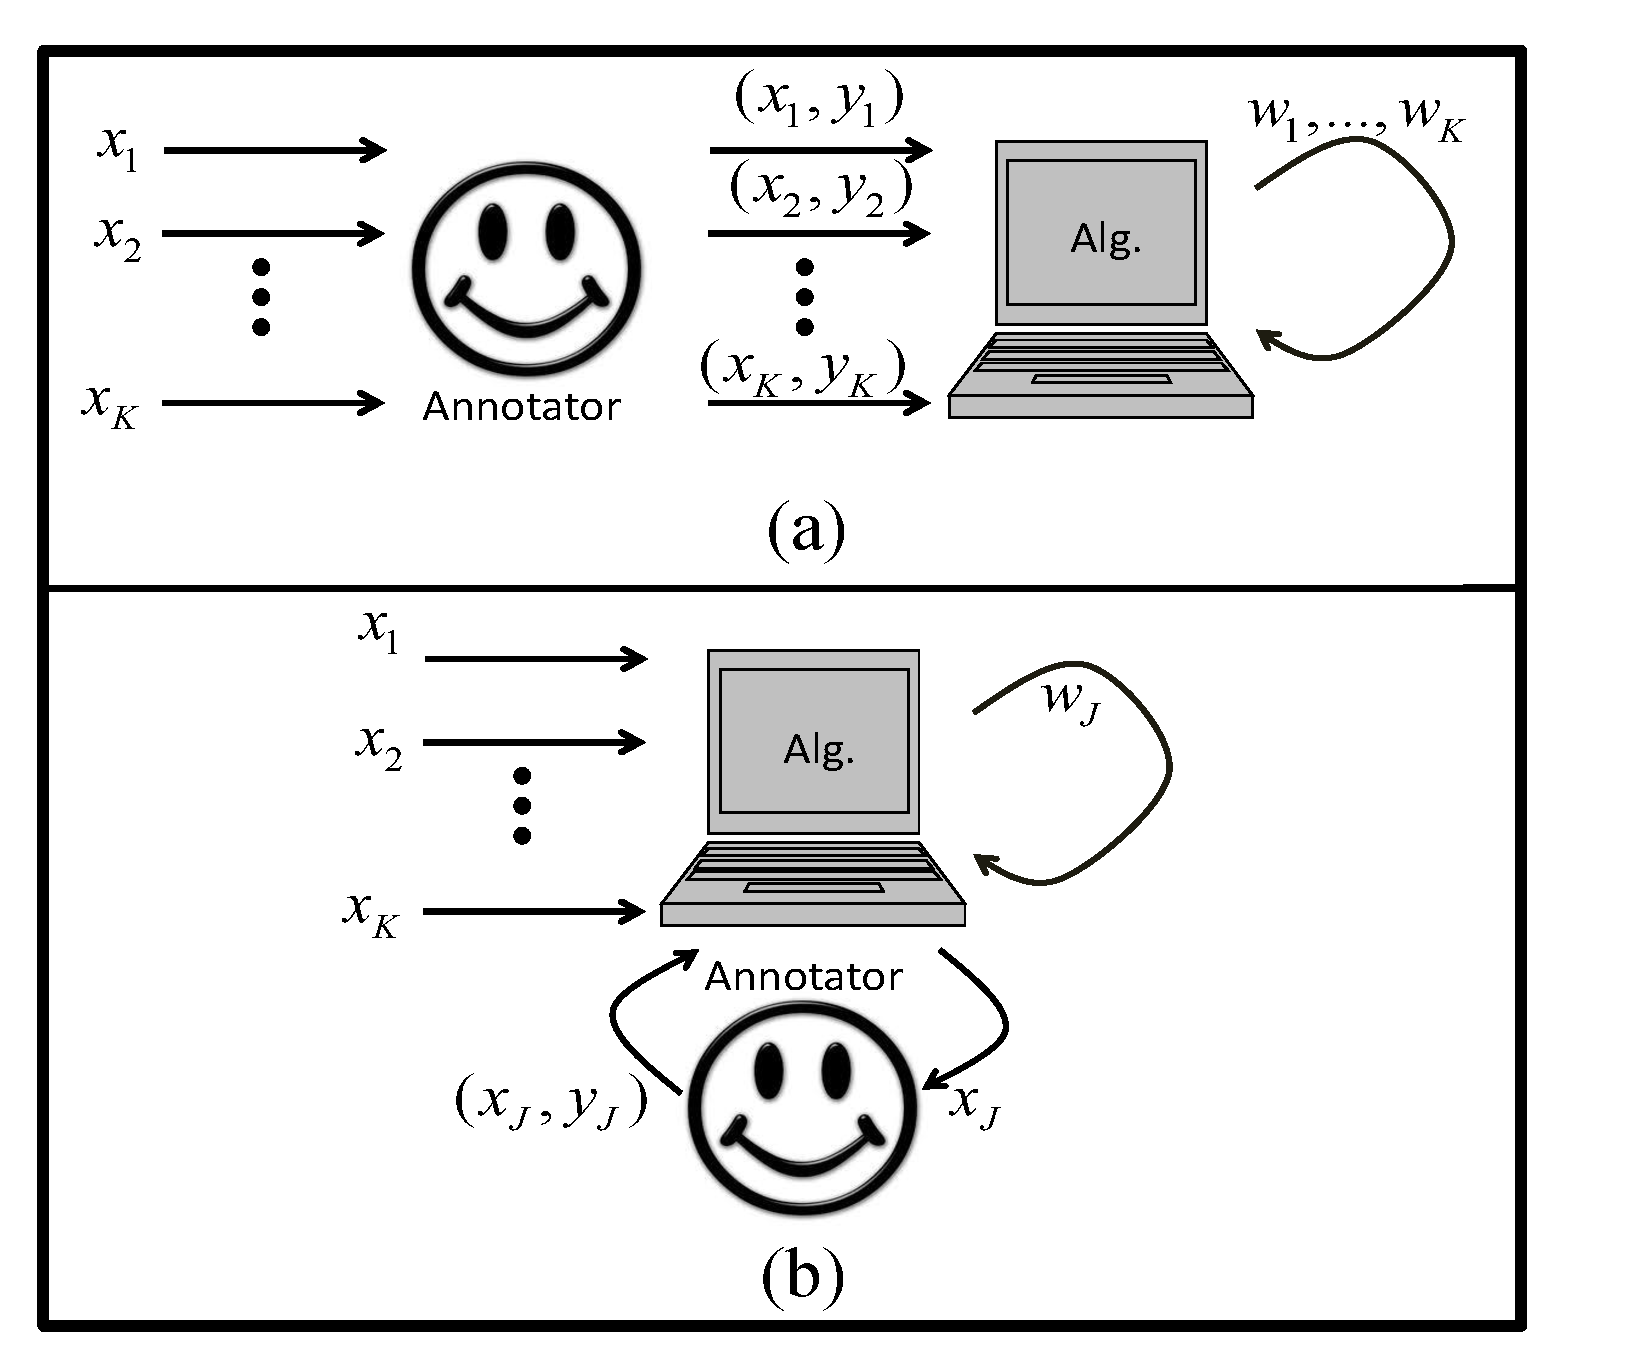
\includegraphics[width=0.5\textwidth]{figs/SHAMPO_illustration.eps}
\caption{Illustration of a single iteration of  multi-task algorithms (a) standard setting, shared annotator labels all inputs, and algorithms update models. (b) SHAMPO algorithm couples labeling annotation and learning process, and synchronizes a single annotation per round.}
\label{fig:ilustration}
\end{centering}
\end{figure}



\chapter{SHMPO (SHared Annotator for Multiple Problems) Algorithms}

I this chapter, we describe algorithms for multi-task learning with
a shared annotator setting, that uses linear models. We start with a basic first order SHAMPO algorithm 
which is based on the perceptron algorithm 
and continue to number of algorithms that extends the basic one. Two steps are
yet to be specified: how to pick a task to be labeled at each round and how to
perform an update, once the true label for that task is given.. 

\section{First Order SHAMPO}

We focus here on linear-functions of the form $f(\vx)=\sign(p)$ for the
quantity $p=\vwt\vx$, $\vw\in\reals^d$,  which often called the
\textit{margin}.
Specifically, the algorithm maintains a set of $K$ weight
vectors, $\vwi{i,t},~i\in\braces{1\comdots K}$. On round $t$, the algorithm predicts a label for each
 one of the tasks, $\hyi{i,t}=\sign(\hat{p}_{i,t})$ where $\hat{p}_{i,t}=\vwti{i,t-1}\vxiit$. 
 On rounds for which the label of some task $J_t$ is queried, the algorithm updates the model of the
 queried task only, such that for the rest of the tasks, $i\neq J_t$, we have $\vwi{i,t}=\vwi{i,t-1}$ and no
 update is made for those unqueried tasks.       

We say that the algorithm has a prediction mistake on task $i$ in round $t$ if
$\yi{i,t} \neq \hyi{i,t}$, and denote this event by the indicator $M_{i,t}=1$,
otherwise, if there is no mistake, we set $M_{i,t}=0$. The goal of the
algorithm is to minimize the cumulative mistakes $\sum_t \sum_i
M_{i,t}$. Models are also evaluated using the
{\em Hinge-loss}. Specifically, let $\vui{i}\in\reals^d$ be some vector
associated with problem $i$. We denote the Hinge-loss of it, with respect
to some input-label  pair $\paren{\vxiit,\yiit}$, by
$\lossp{\gamma,i,t}(\vui{i})= \paren{\gamma-\yiit
  \vuti{i}\vxiit}_+$, where, $(x)_+=\max\{x,0\}$, and $\gamma>0$ is
some parameter. The cumulative loss over all tasks and a sequence of
$n$ input steps, is
$ L_{\gamma,n} =L_{\gamma}(\{ \vui{i} \})=\sum_{t=1}^{n} \sum_{i=1}^{K}\ {\lossp{\gamma,i,t}(\vui{i})}$.
We also use the following expected hinge-loss over the random queried choices
of the algorithm, 
\begin{equation*}
\bar{L}_{\gamma,n}=\bar{L}_{ \{ \vui{i}\}}
=\Exp{\sum_{t=1}^n \sum_{i=1}^{K}{M_{i,t}Z_{i,t}\lossp{\gamma,i,t}(\vui{i})}}. 
 \end{equation*}
Now, we proceed by  describing our algorithm and specify how to choose a task to query its label,
 and how to perform an update.
 

In order to select a task to query on, the algorithm uses the absolute value of the margin 
$\hat{p}_{i,t}$. We can see $\abs{\hat{p}_{i,t}}$ as the certainty measure of the label prediction.
 intuitively if $\abs{\hat{p}_{i,t}}$ is small,
then there is uncertainty about the labeling of $\vxi{i,t}$, and vice-versa for 
large values of $\abs{\hat{p}_{i,t}}$. 
Similar argument was used by ~\cite{DBLP:conf/icml/TongK00} for picking an example to be labeled in 
batch active learning. 
Example for the using of the margin as a certainty measure is shown in \figref{fig:margin} which illustrated 
a state of a linear binary classification algorithm of two dimensional problem. 
The circles and crosses represent two different classes, and the separate hyperplane is shown. 
One of the circles examples have lower margin than the other, so its label can easily been replaced 
with the other one.
Prima facie, under this claim, at each point we should query the true label for the task
 that corresponds to the smallest margin.  Yet, if the model $\vwi{i,t-1}$ is not accurate enough, due to
 small number of observed examples, this estimation may be rough, and may lead to a wrong
conclusion. We thus perform an exploration-exploitation strategy, and
query tasks randomly, with a bias towards tasks with low margin
$\vert \hat{p}_{i,t} \vert$. 

\begin{figure}[h]
\begin{centering}
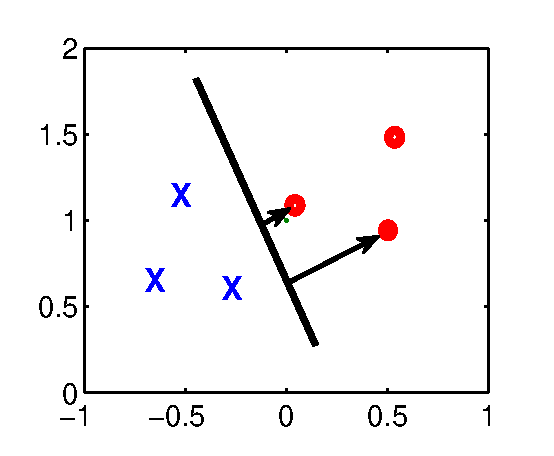
\includegraphics[width=0.5\textwidth]{figs/margin.eps}
\caption{Example for the using of the margin as a certainty measure.}
\label{fig:margin}
\end{centering}
\end{figure}


To the best of our knowledge,
exploration-exploitation usage in this context of choosing an examples
to be labeled (e.g. in settings such as semi-supervised learning or
selective sampling) is novel and new.  In order to get this property, we induced a
distribution over the tasks in the time step $t$, such that the probability to issue a query on the task 
$j$ ( $j=1 \comdots K$) is:

\begin{equation}
\begin{aligned}
\pr{J_t=j}&=\frac{\paren{b+\abs{\hat{p}_{j,t}}-\min_{m=1}^K\abs{\hat{p}_{m,t}}}^{-1}}{D_t}\\
~ \textrm { for } ~
D_{t}&=\sum_{i=1}^{K}{\paren{b+\abs{\hat{p}_{i,t}}-\min_{m}\abs{\hat{p}_{m,t}}}^{-1}}.
\label{eq:prob}
\end{aligned}
\end{equation} 
%
where $m=1 \comdots K$ and $b\geq 0, b\in\reals$ is a tradeoff parameter, between exploration and
exploitation. Clearly, it is a distribution, since $\pr{J_t=j}\geq 0$ and $\sum_j \pr{J_t=j}=1$. 
When we examine the extreme cases  of $b$ we see that  for $b\rightarrow0$
we have $\pr{J_t=j}\rightarrow1$ for the task with minimal margin, $J_t=\arg\min_{i=1}^K\abs{\hat{p}_{i,t}}$,  and $\pr{J_t=j}\rightarrow0$ for all the rest. In this case , pure exploitation is being made. The pure exploration happens when   $b\rightarrow \infty$
, then the distribution is uniform, $ \pr{J_t=j}= 1/K,~~ \forall j $. \figref{fig:probability_example} 
shows an example of this distribution for the case of two tasks ($K=2$) at an arbitrary step $t^*$. 
For visualization purpose, we fix 
$\abs{\hat{p}_{2,t^*}}=0.5$ and see how the probability of task $1$ to be chosen,
 is affected by varying $b$ and $\abs{\hat{p}_{1,t^*}}$ values. 
 Three different vertical areas  can be easily seen 
in the graph. The upper (green) area, where $b>>\max{\braces{\abs{\hat{p}_{1,{t^*}}},\abs{\hat{p}_{2,t{^*}}}}$,
 shows uniform distribution ($\pr{J_{t^*}=2}=\pr{J_{t^*}=1}=1/K=0.5$) 
 which represents the exploration over the tasks.
 In the lower area, the probability is compatible with the exploitation method and is changing between
 probability $1$ in the left, and probability $0$ to the right with a sharp threshold at $\abs{\hat{p}_{1,t^*}}=0.5$, 
 which is very close to the delta distribution $\pr{J_{t^*}=1}=\mathbb{I}\brackets{\hat{p}_{1,{}t^*}<\hat{p}_{2,{t^*}}}$.
 Whereas, the intermediate area, is the exploration-exploitation area that is 
 given by a distribution that is biased toward the lowest margin task.

\begin{figure}[h]
\begin{center}
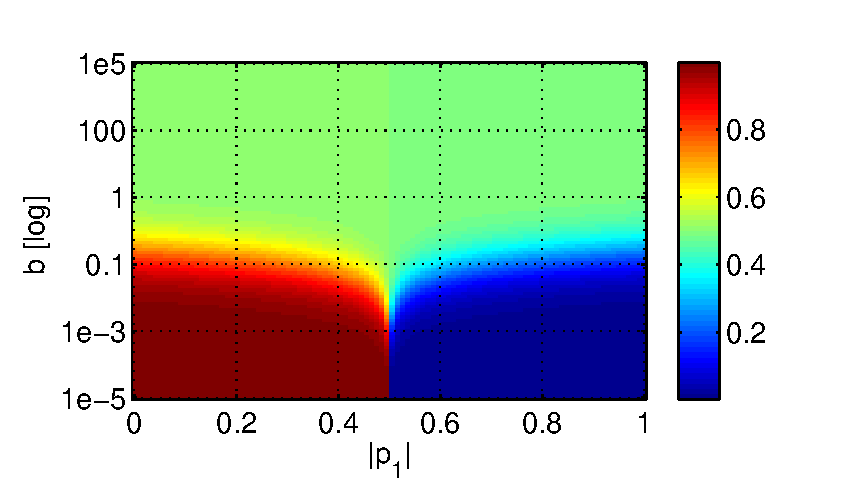
\includegraphics[width=0.80\textwidth]{figs/probability.eps}
\caption{Example of the distribution over 2 tasks.}
\label{fig:probability_example}
\end{center}
\end{figure}

As noted above we denote by $Z_{i,t}=1$ iff $i=J_t$.
The update of the algorithm is performed with the perceptron rule,
that is $\vwi{J_t,t} = \vwi{J_t,t-1}+M_{J_t,t} \, \yi{J_t,t}\,
\vxi{J_t,t}$ and $\vwi{i,t} = \vwi{i,t-1}$ for $i \neq J_t$. 
For simplicity of presentation we write the update for all of the tasks in one term  as, $\vwi{i,t} =
\vwi{i,t-1} + Z_{i,t}\, M_{i,t} \, \yi{i,t}\, \vxi{i,t}$. One can notice that although
this notation uses labels for all tasks,  %(via $M_{i,t}$)
onlythe label of the task $J_t$ is used in practice, as for other tasks $Z_{i,t}=0$.
We call this algorithm {\em SHAMPO} for SHared Annotator for Multiple PrOblems. 
The pseudo-code of this algorithm appears  in ~\algoref{alg:SHAMPO_FO}.

The following theorem states that the expected cumulative number of mistakes
that the algorithm makes, may not be higher than for an algorithm that
observes the labels of all inputs. 
\begin{theorem}
  If SHAMPO algorithm runs on $K$ tasks with $K$ parallel example pair
  sequences
  $(\vxi{i,1},y_{i,1}),\ldots,(\vxi{i,n},y_{i,n})\in\mathbb{R}^d\times\{-1,1\}$,
  $i=1,...,K$ with input parameter $b>0$, then for all $\gamma>0$, all
  $\vui{i}\in\mathbb{R}^d$ and all $n\ge1$, there exists $0<\delta\le K$, such that,
  
\begin{equation}\label{eq:bound_FO_SHAMPO}
\mathbb{E}\left[ \sum_{i=1}^{K}\sum_{t=1}^{n}{M_{i,t}} \right]
\le \frac{\delta}{\gamma}\brackets{\left(1+\frac{X^2}{2b} \right){\bar L}_{\gamma,n}
+\frac{\braces{2b+X^2}^2\tilde{U}^2}{8{\gamma}b}}~,
\end{equation}
 where $X=\max_{i,t}\Vert\vxiit\Vert$,
$\tilde{U}^2=\sum_{i=1}^{K}\normt{\vui{i}}$ and the expectation is over the
random choices of the algorithm.
\end{theorem} \label{thm:FO_theorem}

\begin{algorithm}[h]
\begin{algorithmic}
   \State \textbf{Parameters:}  $b\in\mathbb{R}>0$.
   \State \textbf{Initialize:} $\vwi{i,0}=\vzero$ for $i=1\comdots K$\\
   \For {$t=1,2,\ldots, n$} 
\begin{enumerate}
\nolineskips
\item Observe $K$ instance vectors, $\vxiit$, ($i=1 \comdots K$).
\item Compute margins $\hat{p}_{i,t}=\vwti{i,t-1} \vxiit$.
\item Predict $K$ labels, $\hyi{i,t}=\sign(\hat{p}_{i,t})$.
\item Draw task $J_t$  with the distribution:
\begin{align}
\pr{J_t=j} &=
\frac{\paren{b+\abs{\hat{p}_{j,t}}-\min_{m=1}^K\abs{\hat{p}_{m,t}}}^{-1}}{D_{t}}, \nonumber\\
D_t &=
\sum_i \paren{b+\abs{\hat{p}_{i,t}}-\min_{m=1}^K\abs{\hat{p}_{m,t}}}^{-1}. \nonumber
\end{align}
\item Query the true label ,$\yi{J_t,t}\in\{-1,1\}$.
\item Set the indicator $M_{J_t, t}=1$ iff $\yi{J_t,t} \neq \hyi{J_t,t}$.
\item Update with the perceptron rule:
\begin{align}
&\vwi{J_t,t} = \vwi{J_t,t-1}+M_{J_t,t} \, \yi{J_t,t}\, \vxi{J_t,t}\label{eq:update_rule} \\
&\vwi{i,t} ~~= \vwi{i,t-1}  \textrm{ for } i \neq J_t \nonumber
\end{align}
\end{enumerate}
   \EndFor  
   \State {\bf Output}: $\vwi{i,n}$ for $i=1 \comdots K$.
\end{algorithmic}
\caption{SHAMPO:\@ SHared Annotator for Multiple PrOblems.}\label{alg:SHAMPO_FO}
\end{algorithm}

\begin{proof}
Fix $n$ examples sequences, $(\vxi{i,1},y_{i,1}),\ldots,(\vxi{i,n},y_{i,n})$ for each one of the $K$ tasks. 
Let $t$ be certain trial and $i$ to be an update task on this trial, such that $M_{i,t}=1$. 
We can write,
\begin{align*}
\gamma-\lossp{\gamma,i,t}(\vu_i)&=\gamma-\paren{\gamma-y_{i,t}\vu_i^T\vxiit}_+\\
 ~&\le~  y_{i,t}\vu_i^{T}\vxiit \\
&= y_{i,t}\paren{\vu_i+\vwi{i,t-1}-\vwi{i,t-1}}^{T}\vxiit\\
&= y_{i,t}\vwi{i,t-1}^{T}\vxiit+\paren{\vu_i-\vwi{i,t-1}}^{T}y_{i,t}\vxiit\\
&= y_{i,t}\vwi{i,t-1}^{T}\vxiit+\paren{\vu_i-\vwi{i,t-1}}^{T}\paren{\vwi{i,t}-\vwi{i,t-1}}\\
&=  y_{i,t}\vwi{i,t-1}^{T}\vxiit+\frac{1}{2}{\normt{\vu_{i}-\vwi{i,t-1}}}
        -\frac{1}{2}{\normt{\vu_i-\vwiit}}+\frac{1}{2}{\normt{\vwi{i,t-1}-\vwiit}}\\
&=  y_{i,t}\hat{p}_{i,t}+\frac{1}{2}{\normt{\vu_{i}-\vwi{i,t-1}}}
        -\frac{1}{2}{\normt{\vu_i-\vwiit}}+\frac{1}{2}{\normt{\vwi{i,t-1}-\vwiit}}~.
\end{align*}

\noindent
The last inequality holds for all $\gamma>0$ and for all
$\vu_i\in\mathbb{R}^d$, so we can replace $\gamma$ and $\vu_i$ by their
scaling $\alpha\gamma$ and $\alpha \vu_i$ respectively, where $\alpha>0$
is a scaling parameter that will be determined shortly. Since the inequality is computed on an update task,
$y_{i,t}\hat{p}_{i,t}\le0$ holds , i.e. $y_{i,t}\hat{p}_{i,t}=-\abs{\hat{p}_{i,t}}$ , and we get

\begin{equation}
\begin{split}
\alpha\gamma  +&\abs{\hat{p}_{i,t}} \le\\
&\alpha\lossp{\gamma,i,t}(\vu_i)+\frac{1}{2}{\normt{\alpha \vu_i-\vwi{i,t-1}}}-\frac{1}{2}{\normt{\alpha \vu_i-\vwiit}}+\frac{1}{2}{\normt{\vwi{i,t-1}-\vwiit}} .\end{split}
\label{eq:FO_introducing_alpha}
\end{equation}

\noindent
Now, in order to generalize the inequality, we multiply it by the indicator $M_{i,t}Z_{i,t}$ , 
which means that the inequality holds for  trials and tasks where there is an update, as stated above.

\begin{equation}
\begin{split}
M_{i,t}&Z_{i,t}{\paren{\alpha\gamma +\abs{\hat{p}_{i,t}}}} \!\le\! M_{i,t}Z_{i,t}\alpha \lossp{\gamma,i,t}(\vu_i)
+\\ &\frac{M_{i,t}Z_{i,t}}{2}\normt{\alpha \vu_i-\vwi{i,t-1}}\!-\!\frac{M_{i,t}Z_{i,t}}{2}\normt{\alpha \vu_i-\vwiit}+
\frac{M_{i,t}Z_{i,t}}{2}\normt{\vwi{i,t-1}-\vwiit}.
\end{split}
\label{eq:label}
\end{equation} 

 \noindent
Yet, in the other cases,  when no update is performed and  $M_{i,t}Z_{i,t}=0$,
the equality $\vwiit=\vwi{i,t-1}$ holds as well, so we can rid off the indicator for any one of the last three 
terms and we have

\begin{equation*}
\begin{split}
M_{i,t}Z_{i,t}{\paren{\alpha\gamma +\abs{\hat{p}_{i,t}}}} \le M_{i,t}&Z_{i,t}\alpha \lossp{\gamma,i,t}(\vu_i)+\\ 
\frac{1}{2}\normt{\alpha \vu_i-\vwi{i,t-1}}&-\frac{1}{2}\normt{\alpha \vu_i-\vwiit}+
\frac{M_{i,t}Z_{i,t}}{2}\normt{\vwi{i,t-1}-\vwiit}.
\end{split}
\end{equation*}

\noindent
Next, we sum the inequality above, over $t$,  recall the facts that
$\vwi{i,0}=0$ and $\normt{\vwi{i,t-1}-\vwiit}\le X^2$ for $X=\max_{i,t}\Vert\vxiit\Vert$ to get,

\begin{equation}
\begin{split}
\sum_{t=1}^{n}{M_{i,t}Z_{i,t}{\paren{\alpha\gamma+\abs{\hat{p}_{i,t}}-\frac{X^2}{2}}}}
\le\alpha\sum_{t=1}^{n}{ M_{i,t}Z_{i,t}
  \lossp{\gamma,i,t}(\vu_i)}&+\frac{\alpha^2}{2}\normt{\vu_i}.
\end{split}
\label{eq:FO_step_1_in_proof}
\end{equation}

\noindent
Substituting $\alpha=(2b+X^2)/2\gamma$ (where $b\in\mathbb{R},~~b>0$)
in ~\eqref{eq:FO_step_1_in_proof}, we get
\begin{equation*}
\begin{split}
\sum_{t=1}^{n}{M_{i,t}Z_{i,t}{\paren{b +\abs{\hat{p}_{i,t}}}}}
\le \frac{2b+X^2}{2\gamma}\sum_{t=1}^{n}{ M_{i,t}Z_{i,t}\lossp{\gamma,i,t}(\vu_i)}
+\frac{\left({2b+X^2}\right)^2}{8{\gamma}^2}\normt{\vu_i}.
\end{split}
\end{equation*} 

\noindent
Now, we subtract a non negative quantity $\sum_{t=1}^{n}M_{i,t}Z_{i,t}
{{\min_j{\abs{\hat{p}_{j,t}}}}}$ from the l.h.s. and get,
\begin{equation}
\begin{split}
\sum_{t=1}^{n}M_{i,t}Z_{i,t}{\paren{b +\abs{\hat{p}_{i,t}}-\min_j{\abs{\hat{p}_{j,t}}}}}&\le\\
\frac{2b+X^2}{2\gamma}\sum_{t=1}^{n}{ M_{i,t}Z_{i,t}}&\lossp{\gamma,i,t}(\vu_i)
+\frac{\left({2b+X^2}\right)^2}{8{\gamma}^2}\normt{\vu_i}.
\label{eq:FO_step_2_in_proof}
\end{split}
\end{equation}

\noindent
At this point we take  the expectation of all the terms. 
Recall that the conditional expectation of $Z_{i,t}$ is 
$(b+|\hat{p}_{i,t}|-\min_j| \hat{p}_{j,t}|)^{-1}/D_{t}$
and that $M_{i,t}$ and $\hat{p}_{i,t}$ are measurable with respect to the $\sigma$-algebra that generated by $Z_1,\ldots,Z_{t-1}$. 
We start with the left term,
\begin{align*}
\begin{split}
&\mathbb{E}\brackets{\sum_{t=1}^{n}M_{i,t}Z_{i,t}{\paren{{b
        +\abs{\hat{p}_{i,t}}}-\min_{j}{\abs{ \hat{p}_{j,t}}}}}}= \\
        &\mathbb{E}\brackets{\mathbb{E}_{t-1}\brackets{{\sum_{t=1}^{n}{M_{i,t}Z_{i,t}{\left({b +\abs{\hat{p}_{i,t}}}-\min_{j}{\abs{\hat{p}_{j,t}}}\right)}}}}}= \\
&\mathbb{E}\brackets{{\sum_{t=1}^{n}M_{i,t}{\left({b +\left\vert{\hat{p}_{i,t}}\right\vert}-\min_{j}{\left\vert \hat{p}_{j,t} \right\vert}\right)}\mathbb{E}_{t-1}\brackets{ Z_{i,t}}}}=\\
&\mathbb{E}\brackets{\sum_{t=1}^{n}{\frac{M_{i,t}}{D_{t}}}}~.
\end{split}
\end{align*}

\noindent
Substituting the last term in the expectation of
\eqref{eq:FO_step_2_in_proof}, % we get,
\begin{equation}
\mathbb{E}\left[ \sum_{t=1}^{n}{\frac{M_{i,t}}{D_{t}}} \right]
\le \frac{2b+X^2}{2\gamma}{\bar
  L}_{\gamma,i,n}(u_i)+\frac{\left({2b+X^2}\right)^2}{8{\gamma}^2}{\left\Vert
    \vui{i} \right\Vert}^2~.
\label{eq:FO_step_3_in_proof}
\end{equation} 

\noindent
Since that the normalization factor is a sum of positive components,
hence $D_t$ is maximal when each of the components gets its maximal
value. This happens when $\left\vert \hat{p}_{m,t}
\right\vert=\left\vert \hat{p}_{j,t} \right\vert ~~  \forall
m,j \in\{1,\ldots K\}$. This allows us to bound the normalization factor as
follows,
\begin{equation*}
D_{t}=\sum_{m=1}^{K}{\left({b+\left\vert \hat{p}_{m,t}
      \right\vert-\min_{j}{\left\vert \hat{p}_{j,t}
        \right\vert}}\right)^{-1}} \le \sum_{m=1}^{K}{b^{-1}}=\frac{K}{b}~.
\end{equation*}


\noindent
Since $M_{i,t}>0 ~\forall{i,t}$, thus there exists $\delta_i\in\reals>0$ such that 
\begin{equation}
\label{eq:FO_introducing_delta}
\mathbb{E}\brackets{\sum_{t=1}^{n}{\frac{M_{i,t}}{D_{t}}}} = 
\frac{b}{\delta_i}\mathbb{E}\brackets{\sum_{t=1}^{n}{M_{i,t}}}.
\end{equation}
and
\begin{equation}
\frac{b}{\delta_i} \geq \min\frac{1}{D_t}  = \frac{1}{\max D_t}  \geq 
\frac{b}{K}~.
\label{eq:FO_bound_on_D}
\end{equation}

\noindent
Which implies that $0<\delta_i\le K$.\\
Plugging ~\eqref{eq:FO_introducing_delta} in ~\eqref{eq:FO_step_3_in_proof} we get,
\begin{equation*}
\frac{b}{\delta_i}\mathbb{E}\left[ \sum_{t=1}^{n}{M_{i,t}} \right]
\le \frac{2b+X^2}{2\gamma}{\bar L}_{\gamma,i,n}(\vui{i})+\frac{\left({2b+X^2}\right)^2}{8{\gamma}^2}{\left\Vert \vui{i} \right\Vert}^2.
\end{equation*}

\noindent
Summing up the last inequality over all $K$ tasks and setting $\delta
= \max_i \delta_i$ yields, 
\begin{equation}
\begin{split}
\frac{1}{\delta}\mathbb{E}\left[ \sum_{i=1}^{K}\sum_{t=1}^{n}{M_{i,t}} \right]
\le\frac{1}{\gamma}\left(1+\frac{X^2}{2b} \right){\bar L}_{\gamma,n}+
\frac{\left({2b+X^2}\right)^2}{8{\gamma}^2b}\sum_{i=1}^{K}{{\left\Vert \vui{i} 
\right\Vert}^2}~,
\end{split}
\label{eq:FO_final_eq_in_proof}
\end{equation}
which concludes the proof.
\QED
\end{proof}

\noindent
One can use the bound to tune the algorithm for an optimal value of
$b$. However, this may not be possible as unfortunately ${\bar L}_{\gamma,n}$ depends
implicitly on the value of $b$\ (Similar issue appears also 
after the discussion of Theorem~1 in a different context by~\cite{cesa2006worst}).

\noindent
Alternatively, we can take a
loose estimate of ${\bar L}_{\gamma,n}$, and replace it with
$L_{\gamma,n}$ (which is $\sim K$ times larger). The optimal value of
$b$ can be now calculated, 
\begin{displaymath}
b=\frac{X^2}{2}{\sqrt{1+\frac{4\gamma L_{\gamma,n}}{U^{2}X^2}}}.
\end{displaymath}
Substituting this value in the bound of ~\eqref{eq:bound_FO_SHAMPO} with
$L_{\gamma,n}$ leads to the following bound, 
\begin{equation*}
\mathbb{E}\brackets{\sum_{i=1}^{K}\sum_{t=1}^{n}{M_{i,t}}}
\le\frac{\delta}{\gamma}\brackets{L_{\gamma,n}+\frac{U^{2}X^2}{2\gamma}+\frac{U^{2}}{2\gamma}\sqrt{1+\frac{4\gamma L_{\gamma,n}}{U^{2}X^2}}}
\end{equation*}
which has the same dependency in the number of inputs $n$ as algorithm
that observes all of them.

We continue now with an analysis of an extension of our
algorithm that allows more than a single query per round. In this setting, the ability  
of the annotator to annotate data instances is less limited. Here, we
allow the algorithm to query $\kappa$ labels at a time ( $\kappa<K$), instead of one. On each
iteration $t$, the modified algorithm samples without repetitions,
$\kappa$ labels to be annotated, and perform the same update as of
\eqref{eq:update_rule}. Formally, on each round we have $\sum_i
Z_{i,t}=\kappa$ for $Z_{i,t}\in\{0,1\}$ where the first task-index to
be queried is
drawn according to ~\eqref{eq:prob}. The second task is drawn from the
same distribution, eliminating the first choice and adjusting the normalization factor, and so on. Once
$\kappa$ problems are drawn, the algorithm receives $\kappa$ labels for
the $\kappa$ corresponding inputs, and updates the $\kappa$ models
according to ~\eqref{eq:update_rule}.

\noindent
\begin{corollary}
  If SHAMPO algorithm gets feedback for $\kappa$ tasks on each round,
  instead of only a single problem, the expected cumulative weighted
  mistakes is bounded as follows
\begin{displaymath}
\mathbb{E}\left[ \sum_{i=1}^{K}\sum_{t=1}^{n}{M_{i,t}} \right] 
\le \frac{1}{C(\kappa,K)}\paren{\frac{1}{\gamma}\left(1+\frac{X^2}{2b} \right){\bar L}^\kappa_{\gamma,n}
+\kappa\frac{\left({2b+X^2}\right)^2}{8{\gamma}^2b}\tilde{U}^2}~,
\end{displaymath}
where $C(\kappa,K) = \sum_{j=K-\kappa+1}^{K}\frac{1}{j}$ , and
${\bar L}^\kappa_{\gamma,n}$ is the expected loss of $K$ models
$\{\vui{i}\}$ over the $\kappa$ instances that are annotated per round
$t$.
\end{corollary}

\noindent
\begin{proof}
We follow the proof of \thmref{thm:FO_theorem} until \eqref{eq:FO_final_eq_in_proof}, recall $\delta_i < K$. We
  repeat the process $\kappa$ times, and get the equivalent inequality
  for sampling $\kappa$ problems without repetitions,
\begin{equation}
\begin{split}
  \paren{\sum_{j=K-\kappa+1}^{K}\frac{1}{j}}\mathbb{E}\left[ \sum_{i=1}^{K}\sum_{t=1}^{n}{M_{i,t}} \right]
\le \frac{1}{\gamma}\left(1+\frac{X^2}{2b} \right){\bar L}^\kappa_{\gamma,n}
+\kappa\frac{\left({2b+X^2}\right)^2}{8{\gamma}^2b} U^2~,
\end{split}
\label{final_eq_k}
\end{equation}
where all expectations are now with respect to the sampling
repetitions, and specifically ${\bar L}^\kappa_{\gamma,n}$ is the
expected loss of a set of linear models $\{ \vui{i} \}$ where $\kappa$
problems are sampled rather than a single one.
\QED

% in \eqref{eq:bound_for_i} we saw a bound for the expectation of the sum of errors for the case of $K$ tasks. After we chose one task and got it's feedback, we want to choose another task to issue a query on in the same way. Now we have $K-1$ tasks and the bound
% \begin{equation}
% \sum_{t=1}^{n}\Exp{M_{i,t}\frac{b}{K-1}}
% \le \frac{2b+X^2}{2\gamma}{\bar L}_{\gamma,i,n}(\vui{i})+\frac{\left({2b+X^2}\right)^2}{8{\gamma}^2}{\left\Vert \vui{i} \right\Vert}^2
% \end{equation}
% when $i\ne J_t$. Now we can choose another task out of the $K-2$ tasks and so on. summing over all of the tasks we get the bound expectation of the weight errors over time and tasks
% \begin{equation}
% \Exp{\sum_{t=1}^{n}\brackets{\sum_{J=1}^{\kappa-1}M_{J,t}\frac{1}{K+1-J}+\sum_{i=\kappa }^{K}M_{i,t}\frac{1}{K+1-\kappa}}}
% \le \frac{2b+X^2}{2b\gamma}{\bar L}_{\gamma,n}+\frac{\left({2b+X^2}\right)^2}{8b{\gamma}^2}U.
% \end{equation}
 
\end{proof}

\noindent
It can be shown that this bound  is a generalized form of \thmref{thm:FO_theorem}. 
For $\kappa=1$ we get the bound of \thmref{thm:FO_theorem} (with $\delta = K$), while for
$\kappa=K$ we have $C(\kappa,K)>\ln(K+1)$, thus recovering the
bound of $K$ Perceptron trained in parallel, with a sightly ($\ln(K+1)$)
worse dependency in the number of tasks.

\section{Kernel-Based SHAMPO}
SHAMPO algorithm can also be used with Kernels in order to get a non linear 
classifiers in case of non separated data set, by transforming the feature vector $\vx$ to $\Phi(\vx)$.
Define the binary parameter $\alpha_{i,t} = Z_{i,t}M_{i,t}$, we can rewrite the weight vector $\vw_{i,t}$ in its 
dual form as a linear combination of the input vectors
\[
\vw_{i,t} = \vw_{i,t-1}+Z_{i,t}M_{i,t}y_{i,t}\vxiit =\sum_{s=1}^t{Z_{i,s}M_{i,s}y_{i,s}\vx_{i,s}} 
= \sum_{s=1}^t{\alpha_{i,s}y_{i,s}\vx_{i,s}}.
\]
Now wee can rid of the weight algorithm and store $\alpha_{i,t}$ values and the relevant input-label pairs. 
Doing that, we get a new representation of the margin
\begin{equation*}
\begin{split}
\hat{p}_{i,t}=\vwti{i,t-1} \vxiit
= \tran{\paren{\sum_{s=1}^t{\alpha_{i,s}y_{i,s}\vx_{i,s}}}}\vxiit 
= &\sum_{s=1}^t{\alpha_{i,s}y_{i,s}\paren{\tran{\vx_{i,s}}\vxiit}}\\
=&\sum_{s=1}^t{\alpha_{i,s}y_{i,s}K(\vx_{i,s},\vxiit)}
\end{split}
\end{equation*}
where $K(\vx,\vv)  = \tran{\Phi(\vx)}\Phi(\vv)$ is the kernel function that represents the inner product of 
a high dimension space. 

\section{Aggressive SHAMPO}

So far, we used the margin to build the distribution over the tasks, but in the update stage,
we used the same regular perceptron update rule, that makes an update only when there is a prediction 
mistake. However, we already said that the margin can tells us about the uncertainty in the prediction, 
so it may be helpful to proceed with this approach in the update stage as well and make the sharp update 
threshold a little bit softer. 

In this  version of SHAMPO algorithm, the update is been preformed not only when there is a mistake, 
but also in the case of correct prediction with low margin, i.e. low certainty. We define this margin to be
$\lambda \in\reals>0$. In addition to the previous mistake indicator, $M_{i,t}$,  we introduce one more 
indicator,  $G_{i,t}$. We keep the notation of  $M_{i,t}=1$ when there is wrong prediction on the task $i$
in round $t$ and $M_{i,t}=0$ otherwise, and set $G_{i,t}=1$ when there is no prediction mistake on the task 
$i$ in round $t$, but the margin is lower than our threshold, i.e. $0<\abs{\hat{p}_{i,t}}<\lambda,$ therefore an
aggressive update takes place, and $G_{i,t}=0$  otherwise. 
An update is performed if either there is a mistake ($M_{J_i,t}=1$) or the margin is
low ($G_{J_i,t}=1$). Note that these events are mutually exclusive thus, for simplicity, we define the update
indicator which is  $U_{i,t}=M_{i,t}+G_{i,t}$. This indicator is  $U_{i,t}=1$ on update trials and  $U_{i,t}=0$
when no update has been made.

\begin{algorithm}[h]
\begin{algorithmic}
   \State \textbf{Parameters:}  $b, \lambda \in\mathbb{R}>0$.
   \State \textbf{Initialize:}  $\vwi{i,0}=\vzero$ for $i=1\comdots K$ \\
   \For {$t=1,2,\ldots, n$} 
\begin{enumerate}
\nolineskips
\item Observe $K$ instance vectors, $\vxiit$, ($i=1 \comdots K$).
\item Compute margins $\hat{p}_{i,t}=\vwti{i,t-1} \vxiit$.
\item Predict $K$ labels, $\hyi{i,t}=\sign(\hat{p}_{i,t})$.
\item Draw problem $J_t$  with the distribution:
\begin{align}
\pr{J_t=j} &=
\frac{\paren{b+\abs{\hat{p}_{j,t}}-\min_{m=1}^K\abs{\hat{p}_{m,t}}}^{-1}}{D_{t}}, ~\nonumber\\
D_t &=
\sum_i \paren{b+\abs{\hat{p}_{i,t}}-\min_{m=1}^K\abs{\hat{p}_{m,t}}}^{-1}. \nonumber
\end{align}
\item Query the true label ,$\yi{J_t,t}\in\{-1,1\}$.
\item Set the indicator $M_{J_t, t}=1$ iff $\yi{J_t,t} \neq \hyi{J_t,t}$.
\item Iff $M_{J_t, t}=0$ and $\abs{p_{J_t,t}}<\lambda$, set  the indicator $G_{J_t,t}=1$
\item For $U_{i,t}=M_{i,t}+G_{i,t}$ update with the perceptron rule:
\begin{align}
&\vwi{J_t,t} = \vwi{J_t,t-1}+U_{J_t,t} \, \yi{J_t,t}\, \vxi{J_t,t}  \nonumber\\
&\vwi{i,t} ~~= \vwi{i,t-1}  \textrm{ for } i \neq J_t \nonumber
\end{align}
\end{enumerate}
   \EndFor  
   \State {\bf Output}: $\vwi{i,n}$ for $i=1 \comdots K$.
\end{algorithmic}
\caption{SHAMPO aggressive perceptron.}
\label{alg:SHAMPO_FO_aggressive}
\end{algorithm}    


  


\begin{theorem}
  If Aggressive SHAMPO algorithm runs on $K$ problems with $K$ parallel example pair
  sequences
  $(\vxi{i,1},y_{i,1}),\ldots,(\vxi{i,n},y_{i,n})\in\mathbb{R}^d\times\{-1,1\}$,
  $i=1,...,K$ with input parameters $b>0$, and $0 \le \lambda \le b/2$ then for all $\gamma>0$, all
  $\vui{i}\in\mathbb{R}^d$ and all $n\ge1$, there exists $0<\delta\le K$, such that,
  
\begin{displaymath}
\begin{split}
\mathbb{E}\left[ \sum_{i=1}^{K}\sum_{t=1}^{n}{M_{i,t}} \right]
\le \frac{\delta}{\gamma}&\brackets{\left(1+\frac{X^2}{2b} \right){\bar L}_{\gamma,n}
+\frac{\left({2b+X^2}\right)^2\tilde{U}^2}{8{\gamma}b}}\\ 
+&\paren{2\frac{\lambda}{b}-1}\mathbb{E}\brackets{\sum_{i=1}^{K}\sum_{t=1}^{n}{G_{i,t}}}~,
\label{bound_aggressive_FO_SHAMPO}
\end{split}
\end{displaymath}
 where $X=\max_{i,t}\Vert\vxiit\Vert$,
$\tilde{U}^2=\sum_{i=1}^{K}\normt{\vui{i}}$ and the expectation is over the
random choices of the algorithm.
\end{theorem} \label{thm:FO_bound_aggressive}

\noindent
The theorem above, states that when the update is aggressive, the bound on the expected number of errors
can be tighter than the non aggressive algorithm because we have added a new term to the bound 
which can be negative.     

In order to achieve tighter bound on the expected cumulative mistakes than we had in the regular SHAMPO 
perceptron algorithm (\thmref{thm:FO_theorem}), we need to restrict the aggressive margin  $\lambda$ 
to be $\lambda\le b/2$ so the last term will be negative. Indeed, one can say that this bound shows that the best choice of $\lambda$ is 
$\lambda=0$, i.e. it seems that aggressive update is not a good idea. However, in such case, 
$G_{i,t}=0,~ \forall i,t$ which means that this would not be the best choice of $\lambda$. 
This discrimination actually shows  that there is a sweet point where $0<\lambda<b/2$ such that the 
bound will be the  tightest as this bound allows . 

\begin{proof}
We follow the proof of $\thmref{thm:FO_theorem}$ on an update trial, reminding that now the update 
indicator is  $U_{i,t}=1, $ until we get,  

\begin{align*}
\gamma-&\lossp{\gamma,i,t}(\vu_i)\le \\
&y_{i,t}\hat{p}_{i,t}+\frac{1}{2}{\normt{\vu_{i}-\vwi{i,t-1}}}
        -\frac{1}{2}{\normt{\vu_i-\vwiit}}+\frac{1}{2}{\normt{\vwi{i,t-1}-\vwiit}}~.
\end{align*}
Whereas in the non aggressive version proof we claimed that $y_{i,t}\hat{p}_{i,t}=-\abs{\hat{p}_{i,t}}$ in an 
update trial, here, it is not true when an aggressive update takes place since we update when the prediction 
is correct as well. For that reason, we  remain with the term $y_{i,t}\hat{p}_{i,t}$ as is for now and we will 
deal with it later. In addition, in this proof,  we change the update indicator from $M_{i,t}$ to $U_{i,t}$. 
Considering these two changes, we proceed the proof until $\eqref{eq:FO_step_2_in_proof}$. Now we have,

\begin{equation}
\begin{split}
\sum_{t=1}^{n}U_{i,t}Z_{i,t}{\paren{b -y_{i,t}\hat{p}_{i,t}-\min_j{\abs{\hat{p}_{j,t}}}}}&\le\\
\frac{2b+X^2}{2\gamma}\sum_{t=1}^{n}U_{i,t}Z_{i,t}&\lossp{\gamma,i,t}(\vu_i)+\frac{\left({2b+X^2}\right)^2}{8{\gamma}^2}\normt{\vu_i}.
\label{eq:step_3_in_proof_agressive}
\end{split}
\end{equation}
 Since the inequality is computed on an update task, there is a need to discriminate between   the two possible options: either 
$y_{i,t}\hat{p}_{i,t}\le0$ holds  when there is prediction mistake ($M_{i,t}=1$), i.e. $y_{i,t}\hat{p}_{i,t}=-\abs{\hat{p}_{i,t}}$  ,  or $0\le y_{i,t}\hat{p}_{i,t}\le\lambda$ holds  when the prediction is correct,  but an aggressive update occurs ($G_{i,t}=1$) and  in that case  $y_{i,t}\hat{p}_{i,t}=\abs{\hat{p}_{i,t}}$.

At this point we take  the expectation of all the terms as before taking under consideration the two cases.  Recall that the conditional expectation of $Z_{i,t}$ is
$(b+|\hat{p}_{i,t}|-\min_j| \hat{p}_{j,t}|)^{-1}/D_{t}$
and that $M_{i,t}$ and $G_{i,t}$ (therefor also $U_{i,t}$) and $\hat{p}_{i,t}$ are measurable with respect to the $\sigma$-algebra that generated by $Z_1,\ldots,Z_{t-1}$. 
We start with the left term,
\begin{align}
\begin{split}
&\mathbb{E}\brackets{\sum_{t=1}^{n}U_{i,t}Z_{i,t}{\paren{b-y_{i,t}\hat{p}_{i,t}-\min_{j}{\abs{ \hat{p}_{j,t}}}}}}\\
&=\mathbb{E}\brackets{\mathbb{E}_{t-1}\brackets{{\sum_{t=1}^{n}{U_{i,t}Z_{i,t}{\left(b-y_{i,t}\hat{p}_{i,t}-\min_{j}{\abs{\hat{p}_{j,t}}}\right)}}}}} \\
&=\mathbb{E}\brackets{{\sum_{t=1}^{n}U_{i,t}{\left({b -y_{i,t}\hat{p}_{i,t}}-\min_{j}{\left\vert \hat{p}_{j,t} \right\vert}\right)}\mathbb{E}_{t-1}\brackets{ Z_{i,t}}}}\\
&=\mathbb{E}\brackets{\sum_{t=1}^{n}\frac{\paren{M_{i,t}+G_{i,t}}}{D_{t}}\frac{\paren{b -y_{i,t}\hat{p}_{i,t}-\min_{j}\abs{\hat{p}_{j,t}}}}{b+\abs{\hat{p}_{i,t}}-\min_{j}{\abs{\hat{p}_{j,t}}}}}\\
&=\mathbb{E}\brackets{\sum_{t=1}^{n}{\frac{1}{D_{t}}\paren{M_{i,t}+\frac{b-\abs{\hat{p}_{i,t}}-\min_{j}{\abs{\hat{p}_{j,t}} }}{b+\abs{\hat{p}_{i,t}}-\min_{j}{\abs{\hat{p}_{j,t}}}}G_{i,t} }}}~.
\label{eq:FO_cond_exp}
\end{split}
\end{align}

\noindent
Substituting the last term in the expectation of
\eqref{eq:step_3_in_proof_agressive} we get,
\begin{equation}
\begin{split}
\mathbb{E}\left[ \sum_{t=1}^{n}{\frac{1}{D_{t}}}\paren{M_{i,t}+\frac{b-\abs{\hat{p}_{i,t}}-\min_{j}{\abs{\hat{p}_{j,t}} }}{b+\abs{\hat{p}_{i,t}}-\min_{j}{\abs{\hat{p}_{j,t}}}}G_{i,t} } \right]
&\le \\ \frac{2b+X^2}{2\gamma}{\bar
  L}_{\gamma,i,n}(u_i)+&\frac{\left({2b+X^2}\right)^2}{8{\gamma}^2}{\left\Vert
    \vui{i} \right\Vert}^2~.
\label{step_3_in_proof_aggressive}
\end{split}
\end{equation} 

\noindent
Now we bound the factor that is multiplied by $G_{i,t}$ using the fact that $G_{i,t}=1$ only when 
$\abs{\hat{p}_{i,t}}<\lambda$ ,
\begin{equation}
\label{eq:bound_on_agressive_multiplier}
\paren{1-2\frac{\lambda}{b}}=\frac{b-2\lambda}{b} \le\frac{b-\abs{\hat{p}_{i,t}}-\min_{j}{\abs{\hat{p}_{j,t}} }}{b+\abs{\hat{p}_{i,t}}-\min_{j}{\abs{\hat{p}_{j,t}}}}\le1.
\end{equation}

\noindent
We can use now \eqref{eq:bound_on_agressive_multiplier} to substitute the left hand 
side of \eqref{step_3_in_proof_aggressive} with the lower term

\begin{equation*}
\mathbb{E}\brackets{
  \sum_{t=1}^{n}{\frac{1}{D_{t}}}\paren{M_{i,t}+\paren{1-2\frac{\lambda}{b}}G_{i,t}}}.
\end{equation*}

\noindent
Since $b/2 \geq \lambda$ we have that
$M_{i,t}+\paren{1-2\frac{\lambda}{b}}G_{i,t}\geq 0$,  and as stated before in \eqref{eq:FO_bound_on_D}, 
there exists $\delta_i\in\reals,~ 0<\delta_i\le K$ such that, 
\begin{equation*}
\mathbb{E}\left[
  \sum_{t=1}^{n}{\frac{1}{D_{t}}}\paren{M_{i,t}+\paren{1-2\frac{\lambda}{b}}G_{i,t}
  } \right]=\frac{b}{\delta_i}\mathbb{E}\left[
  \sum_{t=1}^{n}\paren{M_{i,t}+\paren{1-2\frac{\lambda}{b}}G_{i,t}
  } \right] ~.
\end{equation*}

\noindent
Plugging this in ~\eqref{step_3_in_proof_aggressive} we get,
\begin{equation*}
\begin{split}
\frac{b}{\delta_i}\mathbb{E}\brackets{\sum_{t=1}^{n}{M_{i,t}}}
\le& \frac{2b+X^2}{2\gamma}{\bar L}_{\gamma,i,n}(\vui{i})\\
&+\frac{\left({2b+X^2}\right)^2}{8{\gamma}^2}{\left\Vert \vui{i} \right\Vert}^2+ 
     \frac{b}{\delta_i}\paren{2\frac{\lambda}{b}-1}\mathbb{E}\brackets{\sum_{t=1}^{n}{G_{i,t}}}.
\end{split}
\end{equation*}

\noindent
Summing up the last inequality over all $K$ tasks and setting $\delta
= \max_i \delta_i$ yields,
\begin{equation*}
\begin{split}
\frac{1}{\delta}\mathbb{E}\left[ \sum_{i=1}^{K}\sum_{t=1}^{n}{M_{i,t}} \right]
\le&\frac{1}{\gamma}\left(1+\frac{X^2}{2b} \right){\bar L}_{\gamma,n}\\
&+\frac{\left({2b+X^2}\right)^2}{8{\gamma}^2b}\sum_{i=1}^{K}{{\left\Vert \vui{i} \right\Vert}^2}+ \frac{1}{\delta}\paren{2\frac{\lambda}{b}-1}\mathbb{E}\brackets{\sum_{i=1}^{K}\sum_{t=1}^{n}{G_{i,t}}}
\end{split}
\end{equation*}
Which concludes the proof
\QED
\end{proof}

\section{SHAMPO with Prior Knowledge}

We saw before that $b$ is a tradeoff parameter between  exploitation and uniform  distribution over the 
tasks (exploration). It is possible that we have prior knowledge about the tasks (which tasks are harder than 
the others). In this case, we would like to add this prior knowledge to the distribution such that the 
exploration will be done with a prior distribution. This is especially important in the first steps of the 
algorithms when instead starting in pure uniform exploration (since we initialize our model vectors, $\vwi{i,0}=\vzero$),  
we can start with a reasonable prior distribution.
In order to do that we change the probability to be 

\begin{equation*}
\pr{J_t=j} =
\frac{1}{D_{t}}\frac{a_{j}}{\paren{b+\abs{\hat{p}_{j,t}}-\min_{m=1}^K\abs{\hat{p}_{m,t}}}} \end{equation*}
where $a_j>1~~\forall j\in\braces{1,\ldots,K}$ and  $D_t$ is the normalization factor. 
I fact, the bound on $a_i$ is for the analysis only and even lower nonnegative 
values are acceptable since we normalize it.
We can use this distribution with the SHAMPO perceptron algorithm, but for generalization, we would like to analyze the 
bound of the SHAMPO aggressive perceptron algorithm. 

\begin{theorem}
  If Aggressive SHAMPO algorithm with prior runs on $K$ problems with $K$ parallel example pair
  sequences
  $(\vxi{i,1},y_{i,1}),\ldots,(\vxi{i,n},y_{i,n})\in\mathbb{R}^d\times\{-1,1\}$,
  $i=1,...,K$ with input parameters $b>0$, and $\lambda>0$  and $a_i>1~\forall i\in\braces{1,\cdots,K}$ then for all $\gamma>0$, all
  $\vui{i}\in\mathbb{R}^d$ and all $n\ge1$,
  
\begin{displaymath}
\begin{split}
\mathbb{E}\left[ \sum_{i=1}^{K}\sum_{t=1}^{n}{M_{i,t}} \right]
\le\frac{\sum_{j=1}^Ka_{j}}{\gamma}\brackets{\left(1+\frac{X^2}{2b} \right){\bar L}_{\gamma,n}+
\frac{\left({2b+X^2}\right)^2\tilde{U}^2}{8{\gamma}b}}\\ 
+
\paren{2\frac{\lambda}{b}-1}\mathbb{E}\brackets{\sum_{i=1}^{K}\sum_{t=1}^{n}{a_{i}G_{i,t}}},
\label{bound_FO_SHAMPO_prior}
\end{split}
\end{displaymath}
 where $X=\max_{i,t}\Vert\vxiit\Vert$,
$\tilde{U}^2=\sum_{i=1}^{K}\normt{\vui{i}}$ and the expectation is over the
random choices of the algorithm.
\label{thm:FO_bound_aggressive_prior}
\end{theorem} 
This bound brings an advantage and disadvantage. We can reduce the last term in the bound choosing
 the right weights for $a_i$, but then, we suffer a factor of $\sum_{j=1}^Ka_{j}$ in the rest part of the bound. In 
 addition, now the expected loss is changed a bit to be 
 \begin{equation*}
\bar{L}_{\gamma,n}=\Exp{\sum_{t=1}^n \sum_{i=1}^{K}{U_{i,t}Z_{i,t}\lossp{\gamma,i,t}(\vui{i})}},
 \end{equation*}
 since we update sometimes on a correct prediction.  
\\

\begin{proof}
We follow the proof of ~\thmref{bound_aggressive_FO_SHAMPO} until ~\eqref{eq:step_3_in_proof_agressive}, 
than we take the expectation of this term. First, we take the expectation of the left hand side 
where now the conditional expectation of $Z_{i,t}$ changed to 
\[
\mathbb{E}\brackets{Z_{i,t}}=\frac{1}{D_{t}}\frac{a_{i}}{\paren{b+\abs{\hat{p}_{i,t}}-\min_{m=1}^K\abs{\hat{p}_{m,t}}}}.
\]

\noindent
Doing that, the expectation becomes
\begin{align*}
\begin{split}
&\mathbb{E}\brackets{\sum_{t=1}^{n}U_{i,t}Z_{i,t}{\paren{b-y_{i,t}\hat{p}_{i,t}-\min_{j}{\abs{ \hat{p}_{j,t}}}}}} \\
        &=\mathbb{E}\brackets{\mathbb{E}_{t-1}\brackets{{\sum_{t=1}^{n}{U_{i,t}Z_{i,t}{\left(b-y_{i,t}\hat{p}_{i,t}-\min_{j}{\abs{\hat{p}_{j,t}}}\right)}}}}} \\
&=\mathbb{E}\brackets{\sum_{t=1}^{n}{\frac{a_{i}}{D_{t}}\paren{M_{i,t}+\frac{b-\abs{\hat{p}_{j,t}}-\min_{j}{\abs{\hat{p}_{j,t}} }}{b+\abs{\hat{p}_{j,t}}-\min_{j}{\abs{\hat{p}_{j,t}}}}G_{i,t} }}}~.
\end{split}
\end{align*}

\noindent
Recall that $a_{i} \ge 1 \forall i$, we can bound $M_{i,t} \le M_{i,t}a_{i}$ and get 
\begin{equation}
\begin{split}
\mathbb{E}\left[ \sum_{t=1}^{n}{\frac{1}{D_{t}}}\paren{M_{i,t}+\frac{b-\abs{\hat{p}_{j,t}}-\min_{j}{\abs{\hat{p}_{j,t}} }}{b+\abs{\hat{p}_{j,t}}-\min_{j}{\abs{\hat{p}_{j,t}}}}G_{i,t}a_{i} } \right]
&\le \\ \frac{2b+X^2}{2\gamma}{\bar
  L}_{\gamma,i,n}(u_i)+&\frac{\left({2b+X^2}\right)^2}{8{\gamma}^2}{\left\Vert
    \vui{i} \right\Vert}^2~.
\label{eq:step_3_in_proof_prior}
\end{split}
\end{equation}

\noindent
We use now the same bound as in ~\eqref{eq:bound_on_agressive_multiplier}
and plug it into the left side of the inequality,

\begin{multline*}
\mathbb{E}\brackets{\sum_{t=1}^{n}{\frac{1}{D_{t}}}\paren{M_{i,t}+\paren{1-2\frac{\lambda}{b}}G_{i,t}a_{i} }}
\le \\
\mathbb{E}\left[ \sum_{t=1}^{n}{\frac{1}{D_{t}}}\paren{M_{i,t}+\frac{b-\abs{\hat{p}_{j,t}}-\min_{j}{\abs{\hat{p}_{j,t}} }}{b+\abs{\hat{p}_{j,t}}-\min_{j}{\abs{\hat{p}_{j,t}}}}G_{i,t}a_{i} } \right].
\end{multline*}

\noindent
Since $b/2 \geq \lambda$ we have that
$M_{i,t}+\paren{1-2\frac{\lambda}{b}}G_{i,t}a_{i}\geq 0$, thus there
exists $\delta_i$ such that, 

\begin{multline}
  \label{eq:bound_delta_prior}
\mathbb{E}\left[
  \sum_{t=1}^{n}{\frac{1}{D_{t}}}\paren{M_{i,t}+\paren{1-2\frac{\lambda}{b}}G_{i,t}a_{i}
  } \right]= \\
  \frac{b}{\delta_i}\mathbb{E}\left[
  \sum_{t=1}^{n}\paren{M_{i,t}+\paren{1-2\frac{\lambda}{b}}G_{i,t}a_{i}
  } \right] ~,
\end{multline}

\noindent
and 
\[
\frac{b}{\delta_i} \geq \min\frac{1}{D_t}  = \frac{1}{\max D_t}  \geq \frac{b}{\sum_{j=1}^Ka_{j}}~,
\]
where the last inequality follows from,
\begin{equation*}
D_{t}=\sum_{j=1}^K\frac{a_{j}}{\paren{b+\abs{\hat{p}_{j,t}}-\min_{m=1}^K\abs{\hat{p}_{m,t}}}}\le \frac{\sum_{j=1}^Ka_{j}}{b}.
\end{equation*}

\noindent
The last bound implies that $0<\delta_i\le\sum_{i=1}^Ka_{i  }$.

\noindent
Combining ~\eqref{eq:step_3_in_proof_prior} and ~\eqref{eq:bound_delta_prior} leads to, 
\begin{multline*}
\label{eq:bound_for_i}
\frac{b}{\delta_i}\mathbb{E}\left[ \sum_{t=1}^{n}{M_{i,t}} \right]
\le \frac{2b+X^2}{2\gamma}{\bar L}_{\gamma,i,n}(\vui{i}) 
\\+\frac{\left({2b+X^2}\right)^2}{8{\gamma}^2}{\left\Vert \vui{i} \right\Vert}^2 
+\frac{b}{\delta_i}\paren{2\frac{\lambda}{b}-1}a_{i}\mathbb{E}\brackets{\sum_{t=1}^{n}{G_{i,t}}}.
\end{multline*}

\noindent
Summing up the last inequality over all $K$ tasks and setting $\delta
= \max_i \delta_i$ yields,
\begin{equation*}
\begin{split}
\mathbb{E}\left[ \sum_{i=1}^{K}\sum_{t=1}^{n}{M_{i,t}} \right]
\le&\frac{\delta}{\gamma }\brackets{\left(1+\frac{X^2}{2b} \right){\bar L}_{\gamma,n}+
\frac{\left({2b+X^2}\right)^2}{8{\gamma}b}\sum_{i=1}^{K}{{\left\Vert \vui{i} \right\Vert}^2}}\\ 
&+
\paren{2\frac{\lambda}{b}-1}\mathbb{E}\brackets{\sum_{i=1}^{K}\sum_{t=1}^{n}{a_{i}G_{i,t}}}~,
\end{split}
\end{equation*}
which concludes the proof.
\QED
\end{proof}

\noindent
We see that when this  bound is a global bound for the last two algorithms. 
If we set $a_i=1, ~~\forall i\in\braces{1,\cdots,K}$ we get the same bound as  SHAMPO aggressive 
algorithm and if we update only when a prediction mistake occurs, it means that 
$G_{i,t}=0,~~\forall i\in\braces{a,\cdots,K},t>0$ and we get the bound of  the ordinary 
SHAMPO perceptron algorithm.


\section{Adaptive Parameter SHAMPO}

As it has been proved in the analysis and will be shown in experiments, the algorithm parameter $b$ can tune 
the distribution over the tasks between exploration and exploitation, yet, there is still a need to supply 
the algorithm with this input parameter. So far, all of the tasks sheared the same parameter $b$ which
was determined at the beginning of the algorithm and remained constant during the whole process. 
For this reason, once the initial parameters were supplied, the margin was the only factor that had a varying
influence on the distribution. Now, we would like to suggest another algorithm that allow us to
dominate the distribution using the number of updates for each task. 
We assume as in ~\cite{cesa2006worst} that the algorithm makes more mistakes on harder task than easier one, so a natural choice 
at any time, can be one that set higher probability to the tasks that made more prediction mistakes up to 
the same time. 

The adaptive algorithm is similar to the one in ~\algoref{alg:SHAMPO_FO} with three variations in order to 
comply with the intuition. Here we introduce two more variables per task. First, the scalar 
$N_{i,n} = \sum_{t=1}^n{Z_{i,t}M_{i,t}}$ that holds the number of updates that has been done for the 
$i^{th}$ task  up to the time step $n$.
For simplicity of analysis we will write it in it's recursive way $N_{i,t}=N_{i,t-1}+Z_{i,t}M_{i,t}$.
The second variable is $X_{i,t}$ which is holds at the end of each cycle,  
the maximal norm of the input vectors that were involved in the updates.  
The algorithm still have a parameter $\beta>0 \in\mathbb{R}$ to be 
determined, however, it has less influence on the distribution than the parameter $b$ in ~\algoref{alg:SHAMPO_FO} .
Using those three new parameters, we introduce the adaptive version of $b$
\[
b_{i,t-1}=\beta X_{i,t} \sqrt{1+N_{i,t-1}}
\]
 The adaptive version of the  SHAMPO perceptron algorithm is  described in ~\algoref{alg:SHAMPO_adaptive}. 

\begin{algorithm}[!h]
\begin{algorithmic}
   \State \textbf{Parameters:}  $\beta\in\mathbb{R}>0$.
   \State \textbf{Initialize:} $\vwi{i,0}=\vzero$ for $i=1\comdots K$\\
   \For {$t=1,2, ..., n$} 
   \begin{enumerate}
\nolineskips
\item Observe $K$ instance vectors, $\vxiit$, ($i=1 \comdots K$).
\item Compute margins $\hat{p}_{i,t}=\vwti{i,t-1} \vxiit$.
\item Predict $K$ labels, $\hyi{i,t}=\sign(\hat{p}_{i,t})$.
\item Set $\tilde{X}_{i,t}=\max\paren{X_{i,t-1},\Vert\vxiit\Vert}$
\item Draw task $J_t$  with the distribution:
\begin{align}
\pr{J_t=j} &=
\frac{1}{D_t}\frac{b_{i,t}}{b_{i,t}+\abs{\hat{p}_{j,t}}-\min_{m=1}^K\abs{\hat{p}_{m,t}}},\nonumber\\
D_t &=
\sum_i \frac{b_{i,t}}{b_{i,t}+\abs{\hat{p}_{j,t}}-\min_{m=1}^K\abs{\hat{p}_{m,t}}}.\nonumber
\end{align}
Where $b_{i,t} = \beta \tilde{X}_{i,t}^2\sqrt{1+N_{i,t}}$.
\item Query the true label ,$\yi{J_t,t}\in\{-1,1\}$.
\item Set the indicator $M_{J_t, t}=1$ iff $\yi{J_t,t} \neq \hyi{J_t,t}$.
\item Update model's parameters:
\begin{align*}
&\vwi{J_t,t} = \vwi{J_t,t-1}+M_{J_t,t} \, \yi{J_t,t}\, \vxi{J_t,t} \\
&N_{J_t,t} = N_{J_t,t-1} +M_{J_t,t} \\
&X_{J_t,t} = \tilde{X}_{J_t,t} \\
&\vwi{i,t} = \vwi{i,t-1},~~ N_{i,t} = N_{i,t-1}, ~~X_{i,t} = X_{i,t-1}~~ \textrm{ for } i \neq J_t
\end{align*}
\end{enumerate}   \EndFor  
   \State {\bf Output}: $\vwi{i,n}$ for $i=1 \comdots K$.
\end{algorithmic}
\caption{Adaptive SHAMPO algorithm \label{alg:SHAMPO_adaptive}}
\end{algorithm}

\begin{theorem}
  If adaptive SHAMPO algorithm runs on $K$ tasks with $K$ parallel example pair
  sequences
  $(\vxi{i,1},y_{i,1}),...(\vxi{i,n},y_{i,n})\in\mathbb{R}^d\times\{-1,1\}$,
  $i=1,...,K$ with input parameter $\beta>0$, then for all $\gamma>0$, all
  $\vui{i}\in\mathbb{R}^d$ and all $n\ge1$, there exists $0<\delta\le K$, such that,
  
\begin{displaymath}
\mathbb{E}\brackets{ \sum_{i=1}^{K}\sum_{t=1}^{n}{M_{i,t}}}
\le \delta\brackets{\frac{\delta B^2}{2}+\frac{1}{\gamma}{\bar L}_{\gamma,n}+\frac{KR}{2\beta}
+ B\sqrt{\frac{\delta B^2}{4}+\frac{1}{\gamma}{\bar L}_{\gamma,n}+\frac{KR}{2\beta}}}
\end{displaymath}
 where $R = \max_i{\paren{\Vert u_i\Vert X_i}/{\gamma}}$, $B=\paren{R+\frac{2+3R}{2\beta}}$ and the expectation is over the
random choices of the algorithm.
\end{theorem} \label{thm:adaptive_bound}

 \noindent
 \begin{proof}
The proof here is an extended version of the proof in \thmref{thm:FO_theorem} . 
We start here from ~\eqref{eq:FO_introducing_alpha} and replace the constant scaling parameter, 
formerly $\alpha$, with a time varying factor $c_{i,t-1}/\gamma$, where $c_{i,t}\ge0$  is defined as following 
\begin{equation*}
c_{i,t-1}=\half\paren{\max{\braces{X_{i,t-1},\abs{\abs{\vxiit}}}}}+b_{i,t-1}.
\end{equation*}

\noindent
Plugging the new scaling factor into the 
given inequality we get 
\begin{equation*}
\begin{split}
M_{i,t}Z_{i,t}{\paren{c_{i,t-1} +\abs{\hat{p}_{i,t}}}} \le M_{i,t}&Z_{i,t}\frac{c_{i,t-1}}{\gamma} \lossp{\gamma,i,t}(\vu_i)+\\ 
\frac{1}{2}\normt{\frac{c_{i,t-1}}{\gamma} \vu_i-\vwi{i,t-1}}&-\frac{1}{2}\normt{\frac{c_{i,t-1}}{\gamma} \vu_i-\vwiit}+
\frac{M_{i,t}Z_{i,t}}{2}\normt{\vwi{i,t-1}-\vwiit}.
\end{split}
\end{equation*}

\noindent
From the update rule of the  algorithm we can bound $\normt{\vwi{i,t-1}-\vwiit}\le \normt{\vxiit}$. 
This inequality holds for any time step, in particular for an update iteration. 
Using this bound and dividing the inequality by  $b_{i,t-1}$ yields
\begin{equation}
\begin{split}
M_{i,t}Z_{i,t}&{\paren{\frac{c_{i,t-1} +\abs{\hat{p}_{i,t}}-\normt{\vxiit}/2}{b_{i,t-1}}}} \le M_{i,t}Z_{i,t}\frac{c_{i,t-1}}{b_{i,t-1}}\frac{\lossp{\gamma,i,t}(\vu_i)}{\gamma} \\ 
&+\frac{1}{2b_{i,t-1
}}\paren{\normt{\frac{c_{i,t-1}}{\gamma} \vu_i-\vwi{i,t-1}}-\normt{\frac{c_{i,t-1}}{\gamma} \vu_i-\vwiit}}.
\label{eq:AD_first_step}
\end{split}
\end{equation}

\noindent
Now, we decompose the last term of the inequality to two  differences,
\begin{equation*}
\begin{split}
\frac{1}{2b_{i,t-1}}
\paren{\normt{\frac{c_{i,t-1}}{\gamma} \vu_i-\vwi{i,t-1}}-\normt{\frac{c_{i,t-1}}{\gamma} \vu_i-\vwiit}}= \\
\frac{1}{2b_{i,t-1}}\normt{\frac{c_{i,t-1}}{\gamma} \vu_i-\vwi{i,t-1}}-\frac{1}{2b_{i,t}}\normt{\frac{c_{i,t}}{\gamma} \vu_i-\vwi{i,t}}+\\
\frac{1}{2b_{i,t}}\normt{\frac{c_{i,t}}{\gamma} \vu_i-\vwi{i,t}}-\frac{1}{2b_{i,t-1}}\normt{\frac{c_{i,t-1}}{\gamma} \vu_i-\vwiit}.
\end{split}
\end{equation*}

\noindent
At this point expand the last two terms such that
\begin{equation*}
\begin{split}
\frac{1}{2b_{i,t}}\normt{\frac{c_{i,t}}{\gamma} \vu_i-\vwi{i,t}}&-\frac{1}{2b_{i,t-1}}\normt{\frac{c_{i,t-1}}{\gamma} \vu_i-\vwiit}\\
=&\frac{\normt{\vu_i}}{2\gamma^2}\paren{\frac{c_{i,t}^2}{b_{i,t}}-\frac{c_{i,t-1}^2}{b_{i,t-1}}}+
\frac{\vu_i^T\vwiit}{\gamma}\paren{\frac{c_{i,t-1}}{b_{i,t-1}}-\frac{c_{i,t}}{b_{i,t}}}\\
&+\frac{\normt{\vwiit}}{2}\paren{\frac{1}{b_{i,t}}-\frac{1}{b_{i,t-1}}}.
\end{split}
\end{equation*}

\noindent
We know that by definition, $b_{i,t}$ is non decreasing over time such that the last term is always negative 
and can be waved. In addition,  the definition of $c_{i,t}$  leads to 
\begin{equation*}
\frac{c_{i,t}}{b_{i,t}}=\frac{1}{2\beta\sqrt{1+N_{i,t}}}+1
\end{equation*}
which combining with the fact that $N_{i,t}$ is nondecreasing over time as well, we get the inequality 
\begin{equation*}
\frac{c_{i,t}}{b_{i,t}}\le\frac{c_{i,t-1}}{b_{i,t-1}}.
\end{equation*}

\noindent
Combining these facts and using $Cauchy-Schwarz$ the inequality becomes,
\begin{equation}
\begin{split}
\frac{1}{2b_{i,t}}\normt{\frac{c_{i,t}}{\gamma} \vu_i-\vwi{i,t}}&-\frac{1}{2b_{i,t-1}}\normt{\frac{c_{i,t-1}}{\gamma} \vu_i-\vwiit}\\
\le&\frac{\normt{\vu_i}}{2\gamma^2}\paren{\frac{c_{i,t}^2}{b_{i,t}}-\frac{c_{i,t-1}^2}{b_{i,t-1}}}+
\frac{\Vert\vu_i\Vert~\Vert\vwiit\Vert}{\gamma}\paren{\frac{c_{i,t-1}}{b_{i,t-1}}-\frac{c_{i,t}}{b_{i,t}}}.
\end{split}
\label{eq:AD_difference_of_norm_ineq}
\end{equation}

\noindent
Here, recall that on an update trial $y_{i,t}\vw_{i,t-1}^{T}\vxiit\le0$, we define $X_i=\max_t{\Vert\vxiit\Vert}$ 
and use again the update rule and bound the weight vector norm with the number of updates , 
\begin{equation*}
\begin{split}
\normt{\vwiit}&=\normt{\vw_{i,t-1}+M_{i,t}Z_{i,t}y_{i,t}\vxiit}\\
&=\normt{\vw_{i,t-1}}+ 2M_{i,t}Z_{i,t}y_{i,t}\vw_{i,t-1}^{T}\vxiit+M_{i,t}Z_{i,t}\normt{\vxiit}\\
&\le\normt{\vw_{i,t-1}}+M_{i,t}Z_{i,t}\normt{\vxiit}\\
&\le\normt{\vw_{i,t-1}}+M_{i,t}Z_{i,t}X_i^2
\end{split}
\end{equation*}

\noindent
Applying this inequality recursively, combined with the initial value $\vw_{i,0}=0$ leads us to
\begin{equation}
\Vert\vwiit\Vert\le X_i\sqrt{N_{i,t}}
\label{eq:AD_bound_on_w}
\end{equation}
which holds for any $i$ and $t$. Combining the last inequality into  ~\eqref{eq:AD_difference_of_norm_ineq} we get
\begin{equation}
\begin{split}
\frac{1}{2b_{i,t}}\normt{\frac{c_{i,t}}{\gamma} \vu_i-\vwi{i,t}}-\frac{1}{2b_{i,t-1}}\normt{\frac{c_{i,t-1}}{\gamma} \vu_i-\vwiit}\le\\
\frac{\normt{\vu_i}}{2\gamma^2}\paren{\frac{c_{i,t}^2}{b_{i,t}}-\frac{c_{i,t-1}^2}{b_{i,t-1}}}+
\frac{\Vert\vu_i\Vert~ X_i\sqrt{ N_{i,t}}}{\gamma}\paren{\frac{c_{i,t-1}}{b_{i,t-1}}-\frac{c_{i,t}}{b_{i,t}}}.
\label{eq:AD_difference_of_norm_ineq_2}
\end{split}
\end{equation}

\noindent
We will write now, a simpler bound on the last term. First we note that on $t$ that $M_{i,t}Z_{i,t}=1$, i.e. in the case of update, $N_{i,t}=N_{i,t-1}+1$. Using the bound $\sqrt{1+x}-\sqrt{x}\le\frac{1}{2\sqrt{x}}$, yields 
\begin{equation*}
\begin{split}
\sqrt{N_{i,t}}\paren{\frac{c_{t-1}}{b_{t-1}}-\frac{c_t}{b_t}}&=\frac{\sqrt{N_{i,t}}}{2\beta}\paren{\frac{1}{\sqrt{1+N_{i,t-1}}}-\frac{1}{\sqrt{1+N_{i,t}}}}\\
&=\frac{\sqrt{N_{i,t}}}{2\beta}\paren{\frac{1}{\sqrt{N_{i,t}}}-\frac{1}{\sqrt{1+N_{i,t}}}}\\
&=\frac{1}{2\beta}\frac{\sqrt{1+N_{i,t}}-\sqrt{N_{i,t}}}{\sqrt{1+N_{i,t}}}\\
&\le\frac{1}{4\beta}\frac{1}{\sqrt{N_{i,t}}\sqrt{1+N_{i,t}}}\\
&\le\frac{1}{4\beta}\frac{1}{N_{i,t}}.
\end{split}
\end{equation*} 

\noindent
If $M_{i,t}Z_{i,t}=0$ , the left hand side becomes $0$ because in such case, $c_{i,t}=c_{i,t-1}$ and $b_{i,t}=b_{i,t-1}$, which means that this bound holds for all $i$ and $t$ and we can write it as  
\begin{equation*}
\begin{split}
\sqrt{N_{i,t}}\paren{\frac{c_{t-1}}{b_{t-1}}-\frac{c_t}{b_t}}
&\le\frac{M_{i,t}Z_{i,t}}{4\beta}\frac{1}{N_{i,t}}.
\end{split}
\end{equation*}

\noindent
Plugging the  last bound and ~\eqref{eq:AD_difference_of_norm_ineq_2} into ~\eqref{eq:AD_first_step} gives 
us the next inequality that holds for any $i,t,\gamma>0,$ and $u_i\in\reals^d$,
\begin{equation*}
\begin{split}
M_{i,t}Z_{i,t}&{\paren{\frac{c_{i,t-1} +\abs{\hat{p}_{i,t}}-\normt{\vxiit}/2}{b_{i,t-1}}}} \le M_{i,t}Z_{i,t}\frac{c_{i,t-1}}{b_{i,t-1}}\frac{\lossp{\gamma,i,t}(\vu_i)}{\gamma}\\
&+\frac{1}{2b_{i,t-1}}\normt{\frac{c_{i,t-1}}{\gamma} \vu_i-\vwi{i,t-1}}-\frac{1}{2b_{i,t}}\normt{\frac{c_{i,t}}{\gamma} \vu_i-\vwi{i,t}}\\
&+\frac{\normt{\vu_i}}{2\gamma^2}\paren{\frac{c_{i,t}^2}{b_{i,t}}-\frac{c_{i,t-1}^2}{b_{i,t-1}}}+
\frac{\Vert\vu_i\Vert~ X_i}{\gamma}\frac{M_{i,t}Z_{i,t}}{4\beta}\frac{1}{N_{i,t}}.
\end{split}
\end{equation*}

\noindent
Recall the definition of $c_{i,t}$, we can write $c_{i,t-1}-\normt{\vxiit}/2\ge b_{i,t-1}$ and the ineqality gets the form
\begin{equation*}
\begin{split}
M_{i,t}Z_{i,t}&{\paren{\frac{b_{i,t-1} +\abs{\hat{p}_{i,t}}}{b_{i,t-1}}}} \le M_{i,t}Z_{i,t}\frac{c_{i,t-1}}{b_{i,t-1}}\frac{\lossp{\gamma,i,t}(\vu_i)}{\gamma}\\
&+\frac{1}{2b_{i,t-1}}\normt{\frac{c_{i,t-1}}{\gamma} \vu_i-\vwi{i,t-1}}-\frac{1}{2b_{i,t}}\normt{\frac{c_{i,t}}{\gamma} \vu_i-\vwi{i,t}}\\
&+\frac{\normt{\vu_i}}{2\gamma^2}\paren{\frac{c_{i,t}^2}{b_{i,t}}-\frac{c_{i,t-1}^2}{b_{i,t-1}}}+
\frac{\Vert\vu_i\Vert~ X_i}{\gamma}\frac{M_{i,t}Z_{i,t}}{4\beta}\frac{1}{N_{i,t}}.
\end{split}
\end{equation*}

\noindent
Summing  both sides over $t=1,\cdots,n$, and taking into consideration the initialization,   $w_0=0$ we obtain,
\begin{equation}
\begin{split}
\sum_{t=1}^{n}M_{i,t}Z_{i,t}&{\paren{\frac{b_{i,t-1} +\abs{\hat{p}_{i,t}}}{b_{i,t-1}}}} \le \frac{1}{\gamma}\sum_{t=1}^{n}{M_{i,t}Z_{i,t}\frac{c_{i,t-1}}{b_{i,t-1}}\lossp{\gamma,i,t}(\vu_i)}\\
&+\frac{\normt{\vu_i}}{2\gamma^2}\frac{c_{i,n}^2}{b_{i,n}}-\frac{1}{2b_{i,n}}\normt{\frac{c_{i,n}}{\gamma} \vu_i-\vwi{i,n}}
+\frac{\Vert\vu_i\Vert~ X_i}{4\beta\gamma}\sum_{t=1}^{n}{\frac{M_{i,t}Z_{i,t}}{N_{i,t}}}.
\label{eq:AD_first_sum}
\end{split}
\end{equation}

\noindent
Now, we will bound the terms in the right hand side. The first term can be bounded as following,
\begin{equation*}
\begin{split}
\frac{1}{\gamma}\frac{c_{i,t-1}}{b_{i,t-1}}\lossp{\gamma,i,t}(\vu_i)&=\frac{1}{\gamma}\paren{\frac{1}{2\beta\sqrt{1+N_{i,t-1}}}+1}\lossp{\gamma,i,t}(\vu_i)\\
&\le \frac{1}{2\gamma\beta\sqrt{1+N_{i,t-1}}}\paren{\gamma+\Vert u_i\Vert X_i}+\frac{\lossp{\gamma,i,t}(\vu_i)}{\gamma}\\
&=\frac{1}{2\beta\sqrt{1+N_{i,t-1}}}\paren{1+\frac{\Vert u_i\Vert X_i}{\gamma}}+\frac{\lossp{\gamma,i,t}(\vu_i)}{\gamma}
\end{split}
\end{equation*}

\noindent
Here, we used  the fact that $\lossp{\gamma,i,t}(\vu_i)\le \gamma+\Vert u_i\Vert X_i$.
Now we proceed by bounding the two middle terms of ~\eqref{eq:AD_first_sum} such 
that
\begin{equation*}
\begin{split}
\frac{\normt{\vu_i}}{2\gamma^2}\frac{c_{i,n}^2}{b_{i,n}}-\frac{1}{2b_{i,n}}\normt{\frac{c_{i,n}}{\gamma} \vu_i-\vwi{i,n}}
&=\frac{c_{i,n}u_i^T\vwi{i,n}}{b_{i,n}\gamma}-\frac{\normt{\vw_{i,n}}}{2b_{i,n}}\\
&\le \frac{c_{i,n}u_i^T\vwi{i,n}}{b_{i,n}\gamma}\\
&\le\frac{c_{i,n}}{b_{i,n}}\frac{{\Vert u_i\Vert}~{\Vert\vwi{i,n}\Vert}}{\gamma}\\
&\le\paren{\frac{1}{2\beta\sqrt{1+N_{i,n}}}+1}\frac{{\Vert u_i\Vert}X_i\sqrt{N_{i,n}}}{\gamma},
\end{split}
\end{equation*}
where we used ~\eqref{eq:AD_bound_on_w} in the last step.

\noindent
Putting all together in ~\eqref{eq:AD_first_sum}  gives us
\begin{equation*}
\begin{split}
\sum_{t=1}^{n}M_{i,t}Z_{i,t}&{\paren{\frac{b_{i,t-1} +\abs{\hat{p}_{i,t}}}{b_{i,t-1}}}}\\
\le &\frac{1}{2\beta}\paren{1+\frac{\Vert u_i\Vert X_i}{\gamma}}\sum_{t=1}^{n}{\frac{M_{i,t}Z_{i,t}}{\sqrt{1+N_{i,t-1}}}}
+\frac{1}{\gamma}\sum_{t=1}^{n}{M_{i,t}Z_{i,t}}\lossp{\gamma,i,t}(\vu_i)\\
+&\paren{\frac{1}{2\beta\sqrt{1+N_{i,n}}}+1}\frac{{\Vert u_i\Vert}X_i\sqrt{N_{i,n}}}{\gamma}
+\frac{\Vert\vu_i\Vert~ X_i}{4\beta\gamma}\sum_{t=1}^{n}{\frac{M_{i,t}Z_{i,t}}{N_{i,t}}}.
\end{split}
\end{equation*} 

\noindent
The first and the last sums in the right hand side can get more elegant form. Recall $M_{i,t}Z_{i,t}=1$ implies $N_{i,t}=N_{i,t-1}+1$ , we can write  
\begin{equation*}
\begin{split}
\sum_{t=1}^{n}{\frac{M_{i,t}Z_{i,t}}{\sqrt{1+N_{i,t-1}}}}
=\sum_{t=1}^{n}{\frac{M_{i,t}Z_{i,t}}{\sqrt{N_{i,t}}}}
=\sum_{r=1}^{N_{i,n}}{\frac{1}{\sqrt{r}}} 
\le 2\sqrt{N_{i,n}}.
\end{split}
\end{equation*}

\noindent
Now, we apply the same bound on the second sum, but with more loose bound, \begin{equation*}
\begin{split}
\sum_{t=1}^{n}{\frac{M_{i,t}Z_{i,t}}{N_{i,t}}}
\le\sum_{t=1}^{n}{\frac{M_{i,t}Z_{i,t}}{\sqrt{N_{i,t}}}} 
\le 2\sqrt{N_{i,n}}. 
\end{split}
\end{equation*}

\noindent
Defining $R_i=\paren{\Vert u_i\Vert X_i}/{\gamma}$, and combining the last three bounds together we get
\begin{equation*}
\begin{split}
\sum_{t=1}^{n}M_{i,t}Z_{i,t}&{\paren{\frac{b_{i,t-1} +\abs{\hat{p}_{i,t}}}{b_{i,t-1}}}}\\
\le &\frac{1}{\gamma}\sum_{t=1}^{n}{M_{i,t}Z_{i,t}}\lossp{\gamma,i,t}(\vu_i)
+\frac{1}{\beta}\paren{1+\frac{3R_{i}}{2}}\sqrt{N_{i,n}}
\\
+&\frac{R_i}{2\beta}+R_{i}\sqrt{N_{i,n}}.
\end{split}
\end{equation*}

\noindent
Now, we subtract non negative term from the left side, sum the inequality over all tasks and take 
the expectation.
\begin{equation*}
\begin{split}  
\mathbb{E}&\brackets{\sum_{i=1}^K\sum_{t=1}^{n}M_{i,t}Z_{i,t}{\paren{\frac{b_{i,t-1} +\abs{\hat{p}_{i,t}}-\min_j\abs{\hat{p}_{j,t}}}{b_{i,t-1}}}}}\\
\le &\frac{1}{\gamma}\mathbb{E}\brackets{\sum_{i=1}^K\sum_{t=1}^{n}{M_{i,t}Z_{i,t}}\lossp{\gamma,i,t}(\vu_i)}
+\mathbb{E}\brackets{\sum_{i=1}^K\paren{R_{i}+\frac{2+3R_{i}}{2\beta}}\sqrt{N_{i,n}}}\\
&+\mathbb{E}\brackets{\sum_{i=1}^{K}\frac{R_i}{2\beta}}.
\end{split}
\end{equation*}

\noindent
First we look at the left hand side of the inequality.
\[
\sum_{i=1}^{K}\mathbb{E}&\brackets{\sum_{t=1}^{n}M_{i,t}Z_{i,t}{\paren{\frac{b_{i,t-1} +\abs{\hat{p}_{i,t}}-\min_j\abs{\hat{p}_{j,t}}}{b_{i,t-1}}}}}
= \sum_{i=1}^{K}\mathbb{E}\brackets{\sum_{t=1}^{n}\frac{M_{i,t}}{D_t}}
\]
The bound of $D_t$ now is 
\[
D_t = \sum_{i=1}^K{\frac{b_{i,t-1}}{b_{i,t-1} +\abs{\hat{p}_{i,t}}-\min_j\abs{\hat{p}_{j,t}}}}  
\le K
\]
Since $M_{i,t} > 0 \forall i,t$, thus there exists $\delta_i\in\reals, ~0<\delta_i\le K$  such that
\[
\sum_{i=1}^{K}\mathbb{E}\brackets{\sum_{t=1}^{n}\frac{M_{i,t}}{D_t}} 
= \sum_{i=1}^{K}\frac{1}{\delta_i}\mathbb{E}\brackets{\sum_{t=1}^{n}M_{i,t}}  
\le\frac{1}{\delta}\mathbb{E}\brackets{\sum_{i=1}^{K}\sum_{t=1}^{n}M_{i,t}}  
\]
where $\delta = max_i{\delta_i}$.
Next we handle the middle term of the rhs.
\[
\begin{split}
\mathbb{E}&\brackets{\sum_{i=1}^K\paren{R_{i}+\frac{2+3R_{i}}{2\beta}}\sqrt{N_{i,n}}}
\le \mathbb{E}\brackets{\sum_{i=1}^K\paren{R+\frac{2+3R}{2\beta}}\sqrt{N_{i,n}}} \\
&=\paren{R+\frac{2+3R}{2\beta}}\mathbb{E}\brackets{\sum_{i=1}^K\sqrt{N_{i,n}}},
\end{split}
\]
Where $R=\max_i\paren{\Vert u_i\Vert X_i}/{\gamma}$.
Now, considering that $N_{i,n}$ is non-negative and and exploiting the concavity 
of the square root function we can continue as following
\[
\begin{split}
\mathbb{E}\brackets{\sum_{i=1}^K\sqrt{N_{i,n}}} 
&\le \mathbb{E}\brackets{\sqrt{K\sum_{i=1}^KN_{i,n}}}
=\sqrt{K}\mathbb{E}\brackets{\sqrt{\sum_{i=1}^KN_{i,n}}}\\
&\le \sqrt{K}\sqrt{\mathbb{E}\brackets{\sum_{i=1}^KN_{i,n}}}.
\end{split}
\]

\noindent
Here we used the bound for sum of squares, $\sum_{i=1}^K\sqrt{a_i} \le \sqrt{K\sum_{i=1}^K a_i}$ 
for $a_i\in \reals, a_i\ge0$ combining with Jensen inequality. Moreover, we can 
continue, recall that by definition, $N_{i,n} = \sum_{t=1}^n{Z_{i,t}M_{i,t}}$ and $Z_{i,t}M_{i,t} \le M_{i,t}$ 
such that 
\[
\sqrt{K}\sqrt{\mathbb{E}\brackets{\sum_{i=1}^KN_{i,n}}} 
\le \sqrt{K}\sqrt{\mathbb{E}\brackets{\sum_{i=1}^K\sum_{t=1}^nM_{i,t}}}.
\]

\noindent
Plugging the result in the inequality, we get
\begin{equation*}
\begin{split}
\frac{1}{\delta}\mathbb{E}&\brackets{\sum_{i=1}^{K}\sum_{t=1}^{n}M_{i,t}}\\
\le &\frac{1}{\gamma}\mathbb{E}\brackets{\sum_{i=1}^{K}\sum_{t=1}^{n}{M_{i,t}Z_{i,t}}\lossp{\gamma,i,t}(\vu_i)}
+\mathbb{E}\brackets{\sum_{i=1}^{K}\paren{R_{i}+\frac{2+3R_{i}}{2\beta}}\sqrt{N_{i,n}}}
+\mathbb{E}\brackets{\sum_{i=1}^{K}\frac{R_i}{2\beta}}\\
\le & \frac{1}{\gamma}{\bar L}_{\gamma,n}+\paren{R+\frac{2+3R}{2\beta}}\sqrt{K}\sqrt{\mathbb{E}\brackets{\sum_{i=1}^K\sum_{t=1}^nM_{i,t}}}
+\frac{KR}{2\beta}
\end{split}
\end{equation*}
which is quadratic inequality in  $\sqrt{\mathbb{E}\brackets{ \sum_{i=1}^{K}\sum_{t=1}^{n}{M_{i,t}} }$. 

\noindent
Solving this equation and gives us the bound for  the cumulative mistakes
\[
\mathbb{E}\brackets{ \sum_{i=1}^{K}\sum_{t=1}^{n}{M_{i,t}}}
\le \delta\brackets{\frac{\delta B^2}{2}+\frac{1}{\gamma}{\bar L}_{\gamma,n}+\frac{KR}{2\beta}
+ B\sqrt{\frac{\delta B^2}{4}+\frac{1}{\gamma}{\bar L}_{\gamma,n}+\frac{KR}{2\beta}}}
\]
where $B=\paren{R+\frac{2+3R}{2\beta}}$.
\QED
\end{proof}

\chapter{Second Order SHAMPO}

% \section{second order aggressive}
% 
%   \begin{algorithmic}
%     \State \textbf{Parameters:}  $c\in\mathbb{R}>0$.\\ 
%     \State \textbf{Initialize:} $\vwi{i,0}=\vzero$, $A_0=I$ \\
%     \For {$t=1,2, ..., n$} 
%       
% \begin{enumerate}
% \nolineskips
% \item Observe $K$ instance vectors, $\vxiit$, ($i=1 \comdots K$).
% \item Compute  $\hat{p}_{i,t}=\vxiit^T \paren{A_{i,t-1}+\vxiit\vxiit^T}^{-1}\vw_{i,t-1}$.
% \item Predict $K$ labels, $\hyi{i,t}=\sign(\hat{p}_{i,t})$.
% \item Compute $r_i = \vxiit^T A_{i,t-1}^{-1}\vxiit$.
% \item Draw problem $J_t$  with the distribution:
% \begin{align}
% \pr{J_t=j} &=
% \frac{1}{D_{t}}\frac{2c}{2c+\paren{\Theta\paren{\abs{\hat{p}_{j,t}},r_{j,t}}}_+}, \nonumber\\
% D_t &=2c
% \sum_i \paren{2c+\paren{\Theta\paren{\abs{\hat{p}_{i,t}},r_{i,t}}}_+}^{-1}. \nonumber
% \end{align}
% %Where $m,i\in\{1,...,K\}$ and $D_t$ is the normalization factor. Set $Z_{J,t}=1,~Z_{i,t}=0 , ~\forall i\ne J $.
% If  \Theta\paren{\abs{\hat{p}_{J_t,t}},r_{i,t}}\ge0 \Then
%         
%         if $y_{J_t,t}\ne{\hat{y}_{J_t,t}$ set $U_{J_t,t}=1$.
%         
%         end if 
% 
% else
% 
% set $U_{J_t,t}=1$.
% 
% end if.
% 
% \item Update:
% \begin{align}
% &\vwi{J_t,t} = \vwi{J_t,t-1}+U_{J_t,t}\,  \vxi{J_t,t}  \yi{J_t,t}\,\label{perc_update}\\
% &A_{J_t,t}=A_{J_t,t-1}+ U_{J_t,t}\vxi{J_t,t}\vxi{J_t,t}^T\nonumber
% \end{align}
% \end{enumerate}
% \EndFor  
% \State {\bf Output}: $\vwi{i,n}$ for $i=1 \comdots K$.
% \end{algorithmic}\\

% \caption{Second order aggressive SHAMPO. \label{alg:SHAMPO}}
% \end{figure}        
%\end{algorithm}


This algorithm and proof builds on the second order selective sampling by Cesa-Bianchi et al ~\cite{cesa2006worst} define the function
\begin{equation}
\Theta\paren{\abs{\hat{p}_{i,t}},r_{i,t}}=\paren{1+r_{i,t}}\hat{p}_{i,t}^2+2\abs{\hat{p}_{i,t}}-\frac{r_{i,t}}{1+r_{i,t}}
\end{equation}

In order to understand the way that the aggressive update works, there is a need to examine the function $\Theta\paren{\abs{\hat{p}_{i,t}},r_{i,t}}$. One can see that this function is quadratic in $\hat{p}_{i,t}$ , such that it becomes negative in a close interval. Solving this quadratic form, shows that 
\begin{equation}
\Theta\paren{\abs{\hat{p}_{i,t}},r_{i,t}}\le0 \Leftrightarrow \abs{\hat{p}_{i,t}}\le\theta({r_{i,t}})=\frac{-1+\sqrt{1+r_{i,t}}}{1+r_{i,t}}.
\end{equation}
 The last equation shows that the condition on the function $\Theta\paren{\abs{\hat{p}_{j,t}},r_{j,t}}$ can be translated to threshold on the margin. First, a task is chosen according to the distribution above, then, for margin that is less the threshold, an aggressive update will be issued whereas for margin that is bigger than that, the algorithm will performed update only when there is a prediction error. For 
all the rest of the task that were not chosen, no update is issued. For now, we would like to analyse the possibilities for one task in a certain iteration. There are two extreme cases: First, when the the algorithm has not get yet input examples the similar to the current one, which cause the maximal uncertainty i.e., $r_{i,t}=1$. In this case,  the aggressiveness threshold is maximal as well, and we get $\max{\theta({r_{i,t}})}=\frac{-1+\sqrt{2}}{2}\approx0.21$ and an aggressive update will be issued only when the margin is less than this value. Another interesting case is when we saw the same example many times before, such the uncertainty in the prediction now is relatively low, which means $r_{i,t}\approx0$. In this scenario, the aggressive update will be issued only when the margin is zero, $\hat{p}_{i,t}=0$. 
\\

\begin{proof} 
\\ 
Before proofing the Thm. we will use the next inequality. define $x\in[0,1]$
\begin{equation}
\sqrt{1-x}+\sqrt{1+x}\le2.
\label{technical_inequality}
\end{equation}
From the concavity of $\sqrt{1+x}$ we see that $\sqrt{1+x}\le1+\half x$. using this inequality twice, we get $\sqrt{1-x}+\sqrt{1+x}\le1-\half x+1+\half x=2$.

Define 
\begin{equation*}
\Phi_{i,t}(\vu_i)=\half\normt{\vu_i}+\half\sum_{s=1}^{t}{Z_{i,t}U_{i,t}\paren{y_{i,t}-\vu_i^T\vx_{i,t}}}^2
\end{equation*}
Simlar to the proof of Thm .3 of Cesa-Bianchi et al ~\cite{cesa2006worst} and Forster ????,
\begin{equation*}
\begin{split}
\half Z_{i,t}U_{i,t}\paren{y_{i,t}-\hat{p}_{i,t}}^{2}= &\inf_{\vu_i}{\Phi_{i,t+1}}(\vu_i)-\inf_{\vu_i}{\Phi_{i,t}}(\vu_i)+\frac{Z_{i,t}U_{i,t}}{2}\vxiit^TA_{i,t}^{-1}\vxiit\\
&-\frac{Z_{i,t}U_{i,t}}{2}\vxiit^TA_{i,t-1}^{-1}\vxiit\hat{p}_{i,t}^2\\
=&\inf_{\vu_i}{\Phi_{i,t+1}}(\vu_i)-\inf_{\vu_i}{\Phi_{i,t}}(\vu_i)+\frac{Z_{i,t}U_{i,t}}{2}\frac{r_{i,t}}{1+r_{i,t}}-\frac{Z_{i,t}U_{i,t}}{2}r_{i,t}\hat{p}_{i,t}^2
\end{split}
\end{equation*} 
Now, we sum up the equation over $t$,
 
\begin{equation*}
\begin{split}
\half \sum_{t=1}^{n}Z_{i,t}U_{i,t}\paren{y_{i,t}-\hat{p}_{i,t}}^{2}=& \inf_{\vu_i}{\Phi_{i,n+1}}(\vu_i)+ \sum_{t=1}^{n}\frac{Z_{i,t}U_{i,t}}{2}\frac{r_{i,t}}{1+r_{i,t}}-\sum_{t=1}^{n}\frac{Z_{i,t}U_{i,t}}{2}r_{i,t}\hat{p}_{i,t}^2\\
\le&\half\normt{\vu_i}+\half\sum_{t=1}^{n}{Z_{i,t}U_{i,t}\paren{y_{i,t}-\vu_i^T\vx_{i,t}}}^2+ \sum_{t=1}^{n}\frac{Z_{i,t}U_{i,t}}{2}\frac{r_{i,t}}{1+r_{i,t}}\\&-\sum_{t=1}^{n}\frac{Z_{i,t}U_{i,t}}{2}r_{i,t}\hat{p}_{i,t}^2.
\end{split}
\end{equation*} 
For simplification we will define
\begin{equation*}
A_{i,n}=I+\sum_{t=1}^{n}{Z_{i,t}U_{i,t}}\vxiit\vxiit^T.
\end{equation*}
Expanding the squares we get,
\begin{equation}
\begin{split}
\half \sum_{t=1}^{n}Z_{i,t}U_{i,t}&\paren{\hat{p}_{i,t}^2-2y_{i,t}\hat{p}_{i,t}-\frac{r_{i,t}}{1+r_{i,t}}+r_{i,t}\hat{p}_{i,t}^2}\\
\le& \half\normt{\vu_i}+\sum_{t=1}^{n}{Z_{i,t}U_{i,t}\vu_i^T\vx_{i,t}\vx_{i,t}^T\vu_i}-\sum_{t=1}^{n}{Z_{i,t}U_{i,t}\vu_i^T\vx_{i,t}y_{i,t}}\\
&=\half \vu_i^T\paren{I+\sum_{t=1}^{n}{Z_{i,t}U_{i,t}}\vxiit\vxiit^T}\vu_i-\sum_{t=1}^{n}{Z_{i,t}U_{i,t}\vu_i^T\vx_{i,t}y_{i,t}}\\
&=\half \vu_i^T A_{i,n} \vu_i-\sum_{t=1}^{n}{Z_{i,t}U_{i,t}\vu_i^T\vx_{i,t}y_{i,t}}.
\end{split}
\label{sec_order_1}
\end{equation} 
The vectors $\vu_i$ can be replaced with their scaled version, $c\vu_i$. introducing the trivial inequality, $1-x\le \max\braces{1-x,0}$ we get 
\begin{equation}
\begin{split}
cZ_{i,t}U_{i,t}\paren{1-\vu_i^T\vx_{i,t}y_{i,t}} \le cZ_{i,t}U_{i,t}\max\braces{1-\vu_i^T\vx_{i,t}y_{i,t},0}\\
-cZ_{i,t}U_{i,t}\vu_i^T\vx_{i,t}y_{i,t}\le-cZ_{i,t}U_{i,t}+c \lossp{}\paren{\vu_i^T\vx_{i,t}y_{i,t}}.
\label{sec_order_2}
\end{split}
\end{equation}
Rearranging an plugging \eqref{sec_order_2} and \eqref{sec_order_1} 

\begin{equation}
\begin{split}
\half \sum_{t=1}^{n}Z_{i,t}U_{i,t}&\paren{\hat{p}_{i,t}^2-2y_{i,t}\hat{p}_{i,t}-\frac{r_{i,t}}{1+r_{i,t}}+r_{i,t}\hat{p}_{i,t}^{2}+2c}\\
&\le\frac{c^2}{2} \vu_i^T A_{i,n} \vu_i+c\sum_{t=1}^{n}{Z_{i,t}U_{i,t}\lossp{}\paren{\vu_i^T\vx_{i,t}y_{i,t}}}
\label{sec_order_2}
\end{split}
\end{equation}
Recall that $U_{i,t}=M_{i,t}+G_{i,t}$ we will split the inequality into two different cases. First we will take into consideration the cases when an error update was performed, i.e.$M_{i,t}=1$, in which we have $-y_{i,t}\hat{p}_{i,t}=\abs{\hat{p}_{i,t}}$. In this case we need to consider also two subcases, when $\Theta\paren{\abs{\hat{p}_{i,t}},r_{i,t}}\ge0$   and when $\Theta\paren{\abs{\hat{p}_{i,t}},r_{i,t}}<0$. Beginning with the former subcase, recall that for this case 
$\mathbb{E}_{t-1}\brackets{Z_{i,t}}=\frac{1}{D_{t}}\frac{2c}{2c+\paren{\Theta\paren{\abs{\hat{p}_{j,t}},r_{j,t}}}}$, we get 
\begin{equation*}
\begin{split}
\mathbb{E}&\brackets{Z_{i,t}U_{i,t}\paren{\hat{p}_{i,t}^2-2y_{i,t}\hat{p}_{i,t}-\frac{r_{i,t}}{1+r_{i,t}}+r_{i,t}\hat{p}_{i,t}^{2}+2c}}\\
&=\mathbb{E}\brackets{\mathbb{E}_{t-1}\brackets{Z_{i,t}}U_{i,t}\paren{\hat{p}_{i,t}^2-2y_{i,t}\hat{p}_{i,t}-\frac{r_{i,t}}{1+r_{i,t}}+r_{i,t}\hat{p}_{i,t^{}}^{2}+2c}}\\
&=2c\mathbb{E}\brackets{\frac{1}{D_t}U_{i,t}}.
\end{split}
\end{equation*}
When $\Theta\paren{\abs{\hat{p}_{i,t}},r_{i,t}}<0$  the conditional expectation becomes $\mathbb{E}_{t-1}\brackets{Z_{i,t}}=\frac{1}{D_t}$ and the thus,
\begin{equation*}
\begin{split}
\mathbb{E}&\brackets{Z_{i,t}U_{i,t}\paren{\hat{p}_{i,t}^2-2y_{i,t}\hat{p}_{i,t}-\frac{r_{i,t}}{1+r_{i,t}}+r_{i,t}\hat{p}_{i,t}^{2}+2c}}\\
&=\mathbb{E}\brackets{\mathbb{E}_{t-1}\brackets{Z_{i,t}}U_{i,t}\paren{\hat{p}_{i,t}^2+2\abs{\hat{p}_{i,t}}-\frac{r_{i,t}}{1+r_{i,t}}+r_{i,t}\hat{p}_{i,t}^{2}+2c}}\\
&\ge\mathbb{E}\brackets{\mathbb{E}_{t-1}\brackets{Z_{i,t}}U_{i,t}\paren{-\frac{r_{i,t}}{1+r_{i,t}}+2c}}\\
&\ge 2c \mathbb{E}\brackets{\frac{1}{D_t}U_{i,t}}-\frac{r_{i,t}}{1+r_{i,t}}\mathbb{E}\brackets{\frac{1}{D_t}}.
\end{split}
\end{equation*}
Now we examine the case where an update was performed, but there was no mistake. In this case, $0\le y_{i,t}\hat{p}_{i,t}$ and the aggressive update was performed. Recall the bound on the margin for such case and using \eqref{sec_order_2} ,
we bound the margin as follows\begin{equation*}
0\le y_{i,t}\hat{p}_{i,t}\le \theta({r_{i,t}})=\frac{-1+\sqrt{1+r_{i,t}}}{1+r_{i,t}}.
\end{equation*}
We can bound now,
\begin{equation*}
\begin{split}
\hat{p}_{i,t}^2&-2y_{i,t}\hat{p}_{i,t}-\frac{r_{i,t}}{1+r_{i,t}}+r_{i,t}\hat{p}_{i,t}^{2}+2c\\
&=(1+r_{i,t})\hat{p}_{i,t}^2-2y_{i,t}\hat{p}_{i,t}+\frac{r_{i,t}}{1+r_{i,t}}-2\frac{r_{i,t}}{1+r_{i,t}}+2c\\
&=f(y_{i,t}\hat{p}_{i,t})-2\frac{r_{i,t}}{1+r_{i,t}}+2c
\end{split}
\end{equation*}
\end{proof}          
where $f(y_{i,t}\hat{p}_{i,t})=(1+r_{i,t})\hat{p}_{i,t}^2-2y_{i,t}\hat{p}_{i,t}+\frac{r_{i,t}}{1+r_{i,t}}$ is a quadratic convex function with two non-negative roots $\frac{1\pm\sqrt{1-r_{i,t}}}{1+r_{i,t}}$ and we know that the margin is lower than the smaller root , $y_{i,t}\hat{p}_{i,t}\le\frac{1-\sqrt{1-r_{i,t}}}{1+r_{i,t}}$ which leads to the inequality $f(y_{i,t}\hat{p}_{i,t})\ge0$ so we bound 
\begin{equation*}
\begin{split}
\mathbb{E}&\brackets{Z_{i,t}U_{i,t}\paren{\hat{p}_{i,t}^2-2y_{i,t}\hat{p}_{i,t}-\frac{r_{i,t}}{1+r_{i,t}}+r_{i,t}\hat{p}_{i,t}^{2}+2c}}\\
&=\mathbb{E}\brackets{\mathbb{E}_{t-1}\brackets{Z_{i,t}}U_{i,t}\paren{f(y_{i,t}\hat{p}_{i,t})-2\frac{r_{i,t}}{1+r_{i,t}}+2c}}\\
&\ge\mathbb{E}\brackets{\mathbb{E}_{t-1}\brackets{Z_{i,t}}U_{i,t}\paren{-2\frac{r_{i,t}}{1+r_{i,t}}+2c}}\\
&\ge 2c\mathbb{E}\brackets{\frac{1}{D_t}U_{i,t}}-\frac{2r_{i,t}}{1+r_{i,t}}\mathbb{E}\brackets{\frac{1}{D_t}\frac{2r_{i,t}}{1+r_{i,t}}}.
\end{split}
\end{equation*}
Summarize the results we get,
\begin{equation}
\begin{split}
\half \sum_{t=1}^{n}&\mathbb{E}\brackets{Z_{i,t}U_{i,t}\paren{\hat{p}_{i,t}^2-2y_{i,t}\hat{p}_{i,t}-\frac{r_{i,t}}{1+r_{i,t}}+r_{i,t}\hat{p}_{i,t}^{2}+2c}}\\
&\ge c \sum_{t\in\mathcal{M}}\mathbb{E}\brackets{\frac{1}{D_t}U_{i,t}}+c \sum_{t\in\mathcal{G}}\mathbb{E}\brackets{\frac{1}{D_t}U_{i,t}}\\
&-\half\sum_{t\in\mathcal{A\cap M}}\frac{r_{i,t}}{1+r_{i,t}}\mathbb{E}\brackets{\frac{1}{D_t}}
-\sum_{t\in\mathcal{A\cap G}}\frac{r_{i,t}}{1+r_{i,t}}\mathbb{E}\brackets{\frac{1}{D_t}}
\end{split}
\end{equation}
Combining the result of the last inequality with the expectation of the  \eqref{sec_order_2}, recall that  $\sum_{t\in\mathcal{M}}U_{i,t}=M_i$ , and  $\sum_{t\in\mathcal{G}}U_{i,t}=G_i$ we get,   
\begin{equation*}
\begin{split}
c \sum_{t\in\mathcal{M}}\mathbb{E}\brackets{\frac{1}{D_t}U_{i,t}}+c \sum_{t\in\mathcal{G}}\mathbb{E}&\brackets{\frac{1}{D_t}U_{i,t}}
-\frac{1}{2c}\sum_{t\in\mathcal{A\cap M}}\frac{r_{i,t}}{1+r_{i,t}}\mathbb{E}\brackets{\frac{1}{D_t}}\\
-\frac{1}{c}\sum_{t\in\mathcal{A\cap U}}\frac{r_{i,t}}{1+r_{i,t}}\mathbb{E}\brackets{\frac{1}{D_t}}
\le& \frac{c}{2} \vu_i^T \mathbb{E}\brackets{A_{i,n}} \vu_i+\sum_{t=1}^{n}\mathbb{E}\brackets{{Z_{i,t}U_{i,t}\lossp{}\paren{\vu_i^T\vx_{i,t}y_{i,t}}}}
\end{split}
\end{equation*}

The normalization can also been bound by
\begin{equation*}
\begin{split}
D_{t}=2c\sum_{i=1}^{K}{\left({2c+\paren{\Theta\paren{\abs{\hat{p}_{i,t}},r_{i,t}}}_+}\right)^{-1}}& \le  2c\sum_{m=1}^{K}{\frac{1}{2c}}=K
\end{split}
\end{equation*}
which leads to


\begin{equation*}
\begin{split}
\mathbb{E}\brackets{M_{i}}+ &\mathbb{E}\brackets{G_{i}}
-\frac{1}{2c}\mathbb{E}\sum_{t\in\mathcal{A\cap M}}\brackets{\frac{r_{i,t}}{1+r_{i,t}}}
-\frac{1}{c}\mathbb{E}\sum_{t\in\mathcal{A\cap U}}\brackets{\frac{r_{i,t}}{1+r_{i,t}}}\\
\le& \frac{Kc}{2} \vu_i^T \mathbb{E}\brackets{A_{i,n}} \vu_i+K\sum_{t=1}^{n}\mathbb{E}\brackets{{Z_{i,t}U_{i,t}\lossp{}\paren{\vu_i^T\vx_{i,t}y_{i,t}}}}
\end{split}
\end{equation*}



\begin{equation*}
\begin{split}
\mathbb{E}\brackets{M_{i}}\le&\frac{Kc}{2} \vu_i^T \mathbb{E}\brackets{A_{i,n}} \vu_i+K\sum_{t=1}^{n}\mathbb{E}\brackets{{Z_{i,t}U_{i,t}\lossp{}\paren{\vu_i^T\vx_{i,t}y_{i,t}}}} -\mathbb{E}\brackets{G_{i}}\\
&+\frac{1}{2c}\mathbb{E}\sum_{t\in\mathcal{A\cap M}}\brackets{\frac{r_{i,t}}{1+r_{i,t}}}
+\frac{1}{c}\mathbb{E}\sum_{t\in\mathcal{A\cap U}}\brackets{\frac{r_{i,t}}{1+r_{i,t}}}\\
\le& \frac{Kc}{2} \vu_i^T \mathbb{E}\brackets{A_{i,n}} \vu_i+K\mathbb{E}\brackets{\sum_{t=1}^{n}{Z_{i,t}U_{i,t}\lossp{}\paren{\vu_i^T\vx_{i,t}y_{i,t}}}}-\mathbb{E}\brackets{G_{i}}\\
&+\frac{1}{c}\sum_{t\in\mathcal{A}}\brackets{\frac{r_{i,t}}{1+r_{i,t}}}
\end{split}
\end{equation*}
Now, we can summarize the inequality over all of the tasks,
\begin{equation*}
\begin{split}
\mathbb{E}\brackets{M}\le &\frac{cK}{2}\sum_{i=1}^{K}  \vu_i^T \mathbb{E}\brackets{A_{i,n}} \vu_i+K\mathbb{E}\brackets{\sum_{i=1}^{K}\sum_{t=1}^{n}Z_{i,t}U_{i,t}{\lossp{}\paren{\vu_i^T\vx_{i,t}y_{i,t}}}}-\mathbb{E}\brackets{G}\\
&+\frac{1}{c}\mathbb{E}\sum_{i=1}^{K}\sum_{t\in\mathcal{A}}\brackets{\frac{r_{i,t}}{1+r_{i,t}}}
\end{split}
\end{equation*}
 
\begin{equation*}
\begin{split}
\mathbb{E}\brackets{M}\le &\frac{cK}{2}\sum_{i=1}^{K}  \vu_i^T \mathbb{E}\brackets{A_{i,n}} \vu_i+K{\bar L}_{1,n}-\mathbb{E}\brackets{G}\\
&+\frac{1}{c}\mathbb{E}\sum_{i=1}^{K}\sum_{t\in\mathcal{A}}\brackets{\frac{r_{i,t}}{1+r_{i,t}}}
\end{split}
\end{equation*} 




\chapter{From Multi-task to Contextual Bandits}\label{chap:multiclass}
Although our algorithm is designed for many binary-classification tasks that can be independent, 
it can also be applied in two settings of contextual bandits, when decoupling exploration and 
exploitation is allowed as in ~\cite{DBLP:conf/icml/YuM09,DBLP:conf/icml/AvnerMS12}. 
The problem of this setting is predicting a label $\hat{Y}_t \in\{ 1 \comdots C\}$ given an input $\vxi{t}$. 
As before, the algorithm works in rounds. On round $t$ the algorithm receives an input $\vxi{t}$ and 
outputs  multicalss label $\hat{Y}_t\in\{1 \comdots C\}$. 
Then, it queries for some information about the label via a single binary ``yes-no'' question, and uses the 
feedback to update its model. We consider here two forms of binary questions.

\section{One-vs-Rest}
The first setting is termed {\em one-vs-rest}. The algorithm asks if the true label is some label 
$\bar{Y}_t\in\{ 1 \comdots C\}$, possibly not the predicted label, i.e. it may be the case that 
$\bar{Y}_t \neq\hat{Y}_t$. Given the response whether  $\bar{Y}_t$ is the true label $Y_t$, the algorithm 
updates its models. The reduction we perform is by introducing $K$ tasks, one per class. 
The problem of the learning algorithm for task $i$ is to decide whether the true label is class $i$ or not. 
Given the output of all the binary classifiers, the algorithm generates a single multi-class prediction to be the 
single label for which the output of the corresponding binary classifier is positive. If such class does not 
exist, or there are more than one classes  as such, a random prediction is used, i.e., given an input $\vxi{t}$ 
we define $\hat{Y}_t = \arg\max_i \hyi{i,t}$, where ties are broken arbitrarily. The label to be queried is 
$\bar{Y}_t=J_t$, i.e. the problem index that SHAMPO is querying. We analyze the performance of this 
reduction as a multiclass prediction algorithm.

\begin{corollary}
Assume the SHAMPO algorithm is executed as above with $K=C$ one-vs-rest problems, on a sequence 
$(\vx_1,Y_1),\ldots,(\vx_n,Y_n)\in\mathbb{R}^d\times\{1,...,C\}$, and input parameter $b>0$  and prior 
$1\le a_i\forall i$. Then for all $\gamma>0$ and all $\vui{i}\in\mathbb{R}^d$, there 
exists $0<\delta\le \sum_{i=1}^{C}a_{i}$ such that the expected number of multi-class errors is bounded as follows
 \[
 \begin{split}
 &\mathbb{E}\brackets{\sum_t \1{Y_t \neq \hat{Y}_t}}\\
 &\le \frac{\delta}{\gamma}\brackets{\left(1+\frac{X^2}{2b} \right){\bar L}_{\gamma,n}+
 \frac{\left({2b+X^2}\right)^2U^2}{8{\gamma}b}}
 +\paren{2\frac{\lambda}{b}-1}\mathbb{E}\brackets{\sum_{i=1}^{K}\sum_{t=1}^{n}{a_{i}G_{i,t}}}~,
 \end{split}
 \]


where $\1{I}=1$ if the predicate $I$ is true, and zero otherwise.
\end{corollary}
The corollary follows directly from \thmref{thm:bound_aggressive_prior} by noting that, 
$\1{Y_t \neq \hat{Y}_t} \leq \sum_i M_{i,t}$. That is, there is a multiclass mistake if there is at least one 
prediction mistake of one of the one-vs-rest problems. The closest setting is contextual bandits, yet we 
allow decoupling of exploration and exploitation. Ignoring this decoupling, the 
Banditron algorithm~\cite{kakade2008efficient} is the closest to ours, 
with a regret of $O(T^{2/3})$. Hazan et al~\cite{hazan2011newtron} proposed an algorithm 
with $O(\sqrt{T})$ regret but designed for the $\log$ loss, with coefficient that may be very large, and 
another~\cite{DBLP:journals/ml/CrammerG13} algorithm has $O(\sqrt{T})$ regret with respect to prediction 
mistakes, yet they assumed stochastic labeling, rather than adversarial.


\section{One-vs-One}
In the second setting, termed by {\em one-vs-one}, the algorithm picks two labels 
$\bar{Y}^+_t,\bar{Y}^-_t \in\{1\dots C\}$, possibly both not the predicted label. 
The feedback for the learner is three-fold: it is $\yi{J_t,t}=+1$ if the first alternative is the correct label, 
$\bar{Y}^+_t=Y_t$, $\yi{J_t,t}=-1$ if the second alternative is the correct label, $\bar{Y}^-_t=Y_t$, 
and it is $\yi{J_t,t}=0$ otherwise (in this case there is no error and we set $M_{J_t,t}=0$). 
The reduction we perform is by introducing $K= {C \choose 2}$ tasks, one per pair of classes.  
The goal of the learning algorithm for a task indexed with two labels $(y_1,y_2)$ is to decide 
which one is the correct label, given it is one of the two. Given the output of all (binary) classifiers the 
algorithm generates a single multi-class prediction using a tournament in a round-robin 
approach~\cite{DBLP:journals/jmlr/Furnkranz02}. If there is no clear winner, a random prediction is used. 
We now analyze the performance of this reduction as a multiclass prediction algorithm.

\begin{corollary}
Assume the SHAMPO algorithm is executed as above, with $K={C \choose 2}$ one-vs-one problems, 
on a sequence $(\vx_1,Y_1),\ldots,(\vx_n,Y_n)\in\mathbb{R}^d\times\{1,\ldots,C\}$, and input parameter 
$b>0$ and prior $1\le a_i\forall i$ . Then for all $\gamma>0$ and all $\vui{i}\in\mathbb{R}^d$, 
there exists $0<\delta\le \sum_{i=1}^{C \choose 2}a_{i}$ such that the expected number of multi-class 
errors can be bounded as follows
 \[
 \begin{split}
 &\mathbb{E}\brackets{\sum_t \1{Y_t \neq \hat{Y}_t}}\le \frac{2}{({C \choose 2}-1)/2+1}\times\\
 &\braces{ \frac{\delta}{\gamma}\brackets{\paren{1+\frac{X^2}{2b} }{\bar L}_{\gamma,n}+\frac{\paren{{2b+X^2}}^2U^{2}}{8{\gamma}b}}+\paren{2\frac{\lambda}{b}-1}\mathbb{E}\brackets{\sum_{i=1}^{K}\sum_{t=1}^{n}{a_{i}G_{i,t}}}}
 \end{split}
 \]

%where $\1{I}=1$ if the predicate $I$ is true, and zero otherwise.
\end{corollary}
The corollary follows directly from \thmref{thm:bound_aggressive_prior} by noting that the  multiclass error 
is bounded by the multitask errors with a constant factor as following, 
\[
\1{Y_t \neq \hat{Y}_t} \leq \frac{2}{({C \choose 2}-1)/2+1}\sum_{i=1}^{ {C \choose 2}} M_{i,t}. 
\]
The last fact is derived from ~\cite{allwein2001reducing} analysis of the training error 
with the corresponding hamming distance of the ECOC matrix for the One-vs-One 
setting. Note, that the bound is essentially  independent of $C$ as the coefficient in the bound is upper 
bounded by $4$.
% as in Allwin et al. in 

We conclude this section with two algorithmic modifications, we employed in this setting. 
Currently, when the feedback is zero, there is no update of the weights, because there are no errors.
 This causes the algorithm to effectively ignore such examples, as in these cases the algorithm is not 
 modifying any model, furthermore, if such example is repeated, a problem with possibly ``0'' feedback 
 may be queried again.
%We fix this issue with one of two modifications: In the first one, if the feedback is zero, we modify the model to reduce the chance that the chosen problem, $J_t$, would be chosen again for the same input (i.e. not to make the same wrong-choice of choosing irrelevant problem again). To this end, we modify the weights a bit, to increase the confidence (absolute margin) of the model for the same input, and replace \eqref{perc_update} with,
\[
\vwi{J_t,t} = \vwi{J_t,t-1}+ \1{\yi{J_t,t}\ne0} \, \yi{J_t,t}\, \vxi{J_t,t} +
 \1{\yi{J_t,t}=0} \eta \hyi{J_t,t}\vxi{J_t,t}~,
\]
for some $\eta>0$. In other words, if there is a possible error (i.e. $\yi{J_t,t}\ne0$) the update follows the 
Perceptron's rule. Otherwise, the weights are updated such that the absolute margin will increase, 
as 
\[
\begin{split}
\vert \vwti{J_t,t} \vxi{J_t,t} \vert &= \paren{\vwi{J_t,t-1}+ \eta \hyi{J_t,t}\vxi{J_t,t})^{\top}\vxi{J_t,t}}\\ 
&= \vert \vwti{J_t,t-1}\vxi{J_t,t}+ \eta \sign(\vwti{J_t,t-1}\vxi{J_t,t}) \Vert\vxi{J_t,t}\Vert^2 \vert\\
&=\vert \vwti{J_t,t-1}\vxi{J_t,t}\vert + \eta \Vert\vxi{J_t,t}\Vert^2 >\vert \vwti{J_t,t-1}\vxi{J_t,t}\vert. 
\end{split}
\]
We call this method {\em one-vs-one-weak}, as it performs weak updates for zero feedback. 
The second alternative is not to allow $0$ value feedback, and if this is the case, to set the label to be 
either $+1$ or $-1$, randomly.
%Both alternates are evaluated below.
We call this method {\em one-vs-one-random}.



%\section*{Appendix}
%\addcontentsline{toc}{section}{Appendix}
%For some reason, you need to manually add stared sections to the the index file.

% Put the path to your bib file (or whatever else you use) here
\clearpage
%\bibliographystyle{fullname}
\bibliographystyle{plainnat}
\bibliography{bib}

% ********************** ADD THIS BACK ********************************
%\include{hebrewPart}
% *********************************************************************

% Actually, I found it much easier to have each chapter in a file of its own. Except for the Hebrew part, I put it all together in this example just to make things clear.

\end{document}
